\documentclass[a4paper,12pt]{article}
\title{\heiti 物理海洋学笔记}
\author{\small 2017级海洋科学专业 崔英哲 \\ \small \url{https://github.com/Cuiyingzhe/OUC-Physical-Oceanography-Notes}}
\date{\small 2020.07.06}
\usepackage[UTF8]{ctex}
%\usepackage{indentfirst}
\usepackage{geometry}
\usepackage{amsmath}
\usepackage{booktabs}
\usepackage{tabu}
\usepackage{caption}
%\usepackage{gensymb}
\usepackage{graphicx}
\usepackage{float}
\usepackage{cite}
\usepackage{hyperref}
\usepackage{cases}
\usepackage{esint}
\usepackage{fancyhdr}
\usepackage{CJK}
\usepackage{titlesec}
\usepackage{titletoc}
\usepackage{mathrsfs}
\usepackage{harpoon}
\usepackage{amssymb}
\usepackage{color}
\usepackage{bm}
\usepackage{framed}
\usepackage{setspace}
\usepackage{gensymb}
\usepackage{tikz}
\usepackage{cancel}
\usepackage{multicol}
\newcommand*{\circled}[1]{\lower.7ex\hbox{\tikz\draw (0pt, 0pt)%
    circle (.5em) node {\makebox[1em][c]{\small #1}};}}
%\usepackage[T1]{fontenc}
%\usepackage{mathptmx}
\hypersetup{
	colorlinks=true,
	linkcolor=black,
	citecolor=blue
}
\captionsetup[table]{labelsep=space,font={small}}
\captionsetup[figure]{labelsep=space,font={small}}
\geometry{a3paper,left=4cm,right=4cm,top=4cm,bottom=4cm}
\graphicspath{{C:/Users/Gary/Desktop/OUC-Physical-Oceanography-Notes/figures/}}
\begin{document}
    \maketitle
    \renewcommand*\contentsname{}
	\tableofcontents
    \newpage
    \section{基本方程}
    \subsection{旋转坐标系的速度和加速度}
    \setlength{\parindent}{0pt}
    惯性坐标系:
    静止的或是匀速直线运动的坐标系,固定在恒星上的坐标系可以被看成惯性坐标系.\\
    固定在地球上的坐标系:
    地球对恒星的加速度主要是由地球自转引起的,于是可以把地球当作一个对惯性坐标系作纯粹地转运动的物体.
    \subsubsection{旋转坐标系和惯性坐标系中的速度}
    \begin{figure}[H]
		\centering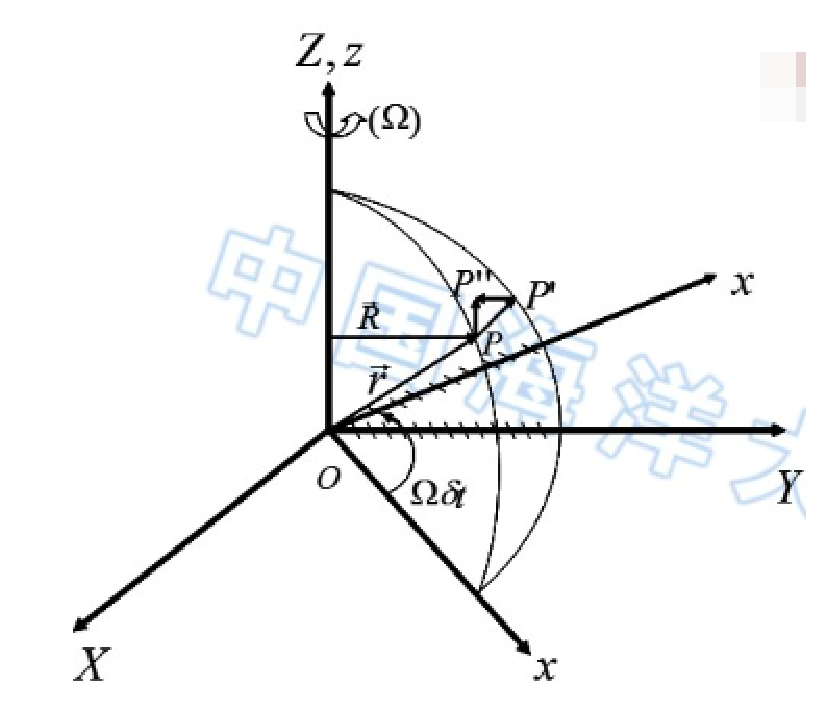
\includegraphics[width=7cm]{1.eps}
		\caption*{}
    \end{figure}
    惯性坐标系($XYZ$)绝对位移:$\vec{pp''}=\vec{V}_a\delta t, \vec{V}_a$为绝对速度\\
    旋转坐标系($xyz$)相对位移:$\vec{p'p''}=\vec{V}\delta t, \vec{V}$为相对速度\\
    $\because \vec{pp''}=\vec{p'p''}+\vec{pp'}$ \\
    $\therefore\vec{V}_a\delta t=\vec{V}\delta t+\vec{V}_e\delta t\Rightarrow\vec{V}_a=\vec{V}+\vec{V}_e$(绝对速度等于相对速度与牵连速度的向量和)\\
    其中,$\vec{V}_e=\vec{\Omega}\times\vec{r}\Rightarrow\vec{V}_a=\vec{V}+\vec{\Omega}\times\vec{r}$
    \[
        \Rightarrow\frac{d_a\vec{r}}{dt}=\frac{d\vec{r}}{dt}+\vec{\Omega}\times\vec{r}
    \]
    \[
        \frac{d_a\vec{A}}{dt}=\frac{d\vec{A}}{dt}+\vec{\Omega}\times\vec{A}
    \]
    \subsubsection{旋转坐标系和惯性坐标系中的加速度}
    令$\vec{A}=\vec{V}_a=\vec{V}_e+\vec{V}=\vec{V}+\vec{\Omega}\times\vec{r}$
    \begin{equation*}
        \begin{aligned} \frac{d \bar{V}_{a}}{d t} &=\frac{d_{a}}{d t}\left(\vec{V}+\vec{V}_{e}\right)=\frac{d_{a}}{d t}(\vec{V}+\vec{\Omega} \times \vec{r}) \\ &=\frac{d}{d t}(\vec{V}+\vec{\Omega} \times \vec{r})+\vec{\Omega} \times(\vec{V}+\vec{\Omega} \times \vec{r}) \\ &=\frac{d \vec{V}}{d t}+\vec{\Omega} \times \vec{V}+\vec{\Omega} \times \vec{V}+\vec{\Omega} \times(\vec{\Omega} \times \vec{r}) \\ &=\frac{d \vec{V}}{d t}+2 \vec{\Omega} \times \vec{V}-\Omega^{2} \vec{R} \end{aligned}
    \end{equation*}
    \subsection{作用在海水微团上的外力 运动方程的向量形式}
    压强梯度力:$\displaystyle\frac{1}{\rho}\nabla p$\\
    分子粘性力(摩擦力):
    \[
        \left\{
        \begin{aligned}
            &F_{x}=\frac{1}{\rho} \mu\left(\frac{\partial^{2} u}{\partial x^{2}}+\frac{\partial^{2} u}{\partial y^{2}}+\frac{\partial^{2} u}{\partial z^{2}}\right)=\frac{\mu}{\rho} \Delta u\\
            &F_{y}=\frac{1}{\rho} \mu\left(\frac{\partial^{2} v}{\partial x^{2}}+\frac{\partial^{2} v}{\partial y^{2}}+\frac{\partial^{2} v}{\partial z^{2}}\right)=\frac{\mu}{\rho} \Delta v\\
            &F_{2}=\frac{1}{\rho} \mu\left(\frac{\partial^{2} w}{\partial x^{2}}+\frac{\partial^{2} w}{\partial y^{2}}+\frac{\partial^{2} w}{\partial z^{2}}\right)=\frac{\mu}{\rho} \Delta w
        \end{aligned}
        \right.
        \Rightarrow \vec{F}=\frac{\mu}{\rho}\Delta \vec{V}=\gamma\Delta\vec{v}
    \]
    重力(地球引力与地球自转产生的惯性离心力的合力):$\displaystyle\vec{g}=-G\frac{M_g}{r^2}\cdot\left(\frac{\vec{r}}{r}\right)$\\
    科氏力:$\displaystyle -2\vec{\Omega}\times\vec{V}$\\
    天体引潮力(受其他天体万有引力与惯性力离心力的合力):$\displaystyle\vec{F_M}=-G\frac{M_M}{L^2}+G\frac{M_M}{D^2}\cdot\left(\frac{\vec{D}}{D}\right)$\\
    由牛顿第二定律和坐标系转换关系:
    \[
        \left\{
        \begin{aligned}
            &\frac{d_{a} \vec{V}_{a}}{d t}=\sum_{i} \vec{F}_{t}\\
            &\frac{d_{a} \vec{A}_{a}}{d t}=\frac{d \vec{V}}{d t}+2 \vec{\Omega} \times \vec{V}-\Omega^{2} \vec{R}
        \end{aligned}
        \right.
    \]
    \[
        \Rightarrow\boxed{\color{red} \frac{d \vec{V}}{d t}=-\frac{1}{\rho} \nabla P-2 \vec{\Omega} \times \vec{V}+\vec{g} +\nu \Delta \vec{V}+\vec{F}_{T}}
    \]
    \subsection{运动方程在球坐标系的标量形式}
    \begin{figure}[H]
        \centering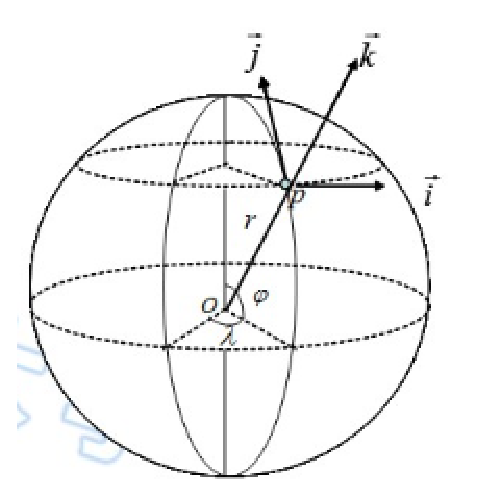
\includegraphics[width=5cm]{2.eps}
        \caption*{}
    \end{figure}
    速度:
    \[
        \vec{V}=u\vec{i}+v\vec{j}+w\vec{k}
    \]
    \[
        \Rightarrow
        \left\{\begin{array}{l}u=r \cos \varphi \frac{d \lambda}{d t} \\ v=r \frac{d \varphi}{d t} \\ w=\frac{d r}{d t}\end{array}\right.
    \]
    加速度:
    \[
        \begin{aligned}
        \frac{d\vec{A}}{dt}&=\frac{\frac{\partial \vec{A}}{\partial t} d t+\frac{\partial \vec{A}}{\partial \lambda} d \lambda+\frac{\partial \vec{A}}{\partial \varphi} d \varphi+\frac{\partial \vec{A}}{\partial r} d r}{dt}\\
        &=\frac{\partial \bar{A}}{\partial t}+\frac{\partial \vec{A}}{\partial \lambda} \frac{d \lambda}{d t}+\frac{\partial \vec{A}}{\partial \varphi} \frac{d \varphi}{d t}+\frac{\partial \vec{A}}{\partial r} \frac{d r}{d t}\\
        &=\frac{\partial \vec{A}}{\partial t}+\frac{u}{r \cos \varphi} \frac{\partial \vec{A}}{\partial \lambda}+\frac{v}{r} \frac{\partial \vec{A}}{\partial \varphi}+w \frac{\partial \vec{A}}{\partial r}
        \end{aligned}
    \]
    \[
        \begin{aligned}
        &\Rightarrow\frac{d}{d t}=\frac{\partial}{\partial t}+u \frac{\partial}{r \cos \varphi \partial \lambda}+v \frac{\partial}{r \partial \varphi}+w \frac{\partial}{\partial r}\\
        &\Rightarrow\boxed{\bm{ \frac{d}{d t}=\frac{\partial}{\partial t}+(\vec{V} \cdot \nabla)}}\\
        &\Rightarrow\boxed{\bm{ \nabla=\frac{\partial}{r \cos \varphi \partial \lambda} \vec{i}+\frac{\partial}{r \partial \varphi} \vec{j}+\frac{\partial}{\partial r} \vec{k}}}
        \end{aligned}
    \]
    \[
        \Rightarrow
        \left\{
            \begin{aligned}
                &\frac{d \vec{i}}{d t}=\frac{\partial \vec{i}}{\partial t}+u \frac{\partial \vec{i}}{r \cos \varphi \partial \lambda}+v \frac{\partial \vec{i}}{r \partial \varphi}+w \frac{\partial \vec{i}}{\partial r}\\
                &\frac{\partial \vec{j}}{d t}=\frac{\partial \vec{j}}{\partial t}+u \frac{\partial \vec{j}}{r \cos \varphi \partial \lambda}+v \frac{\partial \vec{j}}{r \partial \varphi}+w \frac{\partial \vec{j}}{\partial r}\\
                &\frac{d \vec{k}}{d t}=\frac{\partial \vec{k}}{\partial t}+u \frac{\partial \vec{k}}{r \cos \varphi \partial \lambda}+v \frac{\partial \vec{k}}{r \partial \varphi}+w \frac{\partial \vec{k}}{\partial r}
            \end{aligned}
        \right.
    \]
    \newpage
    \[
        \begin{aligned}
            &\frac{d \vec{V}}{d t}=\frac{d u}{d t} \vec{i}+\frac{d v}{d t} \vec{j}+\frac{d v}{d t} \vec{k}+u \frac{d \vec{i}}{d t}+v \frac{d \vec{j}}{d t}+w \frac{d \vec{k}}{d t}\\
            \Rightarrow&\boxed{\color{red}\frac{d \vec{V}}{d t}=\left(\frac{d u}{d t}-\frac{u v t g \varphi}{r}+\frac{u w}{r}\right) \vec{i}+\left(\frac{d v}{d t}+\frac{u^{2} \operatorname{tg} \varphi}{r}+\frac{v w}{r}\right) \vec{j}+\left(\frac{d w}{d t}-\frac{u^{2}+v^{2}}{r}\right)}
        \end{aligned}
    \]
    压强梯度力:
    \[
        \frac{1}{\rho}\nabla p=-\frac{1}{\rho}\left(\frac{1}{r \cos \varphi} \frac{\partial p}{\partial \lambda} \vec{i}+\frac{1}{r} \frac{\partial p}{\partial \varphi} \vec{j}+\frac{\partial p}{\partial r} \vec{k}\right)
    \]
    重力:
    \[
        \vec{g}=-g\vec{k}
    \]
    科氏力:
    \begin{figure}[H]
        \centering 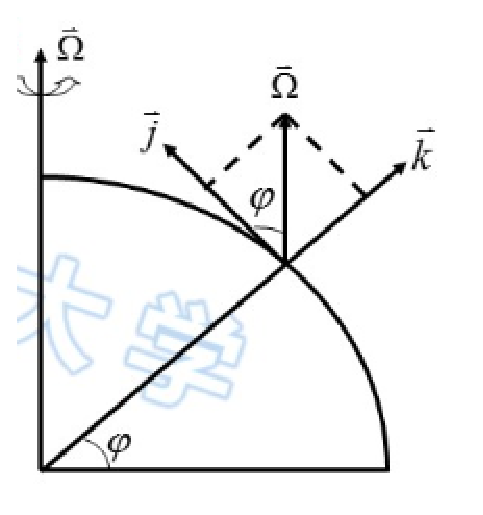
\includegraphics[width=4cm]{3.eps}
        \caption*{}
    \end{figure}
    \vspace{-2cm}
    \[
        \vec{\Omega}=\Omega \sin \varphi \vec{k}+\Omega \cos \varphi \vec{j}
    \]
    \[
        \begin{aligned}
            -2 \vec{\Omega} \times \vec{V}&=-2\left|\begin{array}{ccc}\vec{i} & \vec{j} & \vec{k} \\ 0 & \Omega \cos \varphi & \Omega \sin \varphi \\ u & v & w\end{array}\right|\\
            &=-2[(w \Omega \cos \varphi-v \Omega \sin \varphi) \vec{i}+(u \Omega \sin \varphi) \vec{j}+(-u \Omega \cos \varphi) \vec{k}]
        \end{aligned}
    \]
    \[
        \Rightarrow-2 \vec{\Omega} \times \vec{V}=(f v-\tilde{f} w) \vec{i}-(f u) \vec{j}+(\tilde{f} u) \vec{k}
    \]
    其中,$\displaystyle\left\{\begin{aligned}&f=2\Omega \sin\varphi\\ &\tilde{f}=2\Omega \cos\varphi\end{aligned}\right.$
    \[
        \Rightarrow
        \boxed{
        \left\{
        \begin{aligned}
            &\frac{d u}{d t}=-\frac{1}{\rho} \frac{\partial p}{r \cos \varphi \partial \lambda}+f v-\tilde{f} w+\frac{u v \tan \varphi}{r}-\frac{u w}{r}+\gamma(\Delta \vec{v})_{\lambda}-\frac{1}{r \cos \varphi} \frac{\partial \phi_{T}}{\partial \lambda}\\
            &\frac{d y}{d t}=7 \frac{1}{\rho} \frac{\partial p}{r \partial \varphi}-f u-\frac{u^{2} \tan \varphi}{r}-\frac{v w}{r}+\gamma(\Delta \bar{v})_{\varphi}-\frac{1}{r} \frac{\partial \phi_{T}}{\partial \varphi}\\
            &\frac{d w}{d t}=-\frac{1}{\rho} \frac{\partial p}{\partial r}+\tilde{f} u=g+\frac{u^{2}+v^{2}}{r}+\gamma(\Delta \vec{v})_{r}-\frac{\partial \phi_{T}}{\partial r}
        \end{aligned}
        \right.
        }
    \]
    \subsection{直角坐标系的运动方程}
    略去地球曲率的影响
    \[
        \Rightarrow
        \boxed{
        \left\{
        \begin{aligned}
            &\frac{d u}{d t}=-\frac{1}{\rho} \frac{\partial p}{\partial x}+f v+\tilde{f} w+F_{N \lambda}+F_{T \lambda}\\
            &\frac{d v}{d t}=-\frac{1}{\rho} \frac{\partial p}{\partial x}-f u+F_{N y}+F_{T y}\\
            &\frac{d w}{d t}=-\frac{1}{\rho} \frac{\partial p}{\partial z}+\tilde{f} u-g+F_{N z}+F_{T z}
        \end{aligned}
        \right.
        }
    \]
    \subsection{海水层流运动的基本方程组}
    \subsubsection{连续方程}
    \[
        \frac{\partial \rho}{\partial t}+\nabla \cdot(\rho \vec{V})=0 \Leftrightarrow \frac{d \rho}{d t}+\rho \nabla \cdot \vec{V}=0
    \]
    特别地,对于不可压缩流体:
    \[
        \nabla \cdot \vec{V}=0
    \]
    \subsubsection{盐量扩散方程}
    \[
        \mathop{\frac{\partial}{\partial t} \iiint\limits_{\tau} \rho s d \tau}\limits^{\mbox{盐量增加量}}=\mathop{-\oiint\limits_{\sigma} \rho s V_{n} d \sigma}\limits^{\mbox{平流作用}}+\mathop{-\oiint\limits_{\sigma} S_{n} d \sigma}\limits^{\mbox{分子扩散作用}}
    \]
    \[
        \begin{aligned}
            &\iiint\limits_{\tau} \frac{\partial (\rho s)}{\partial t} d \tau =\iiint\limits_{\tau} \nabla \cdot(\rho s \vec{V}) d \tau -\iiint\limits_{\tau} \nabla \cdot \vec{S} d \tau \\
            \Rightarrow&\frac{\partial(\rho s)}{\partial t}+\nabla \cdot(\rho s \vec{V})+\nabla \cdot \vec{S}=0\\
            \Rightarrow&\rho \frac{\partial s}{\partial t}+s \frac{\partial \rho}{\partial t}+s \nabla \cdot(\rho \vec{V})+\rho \vec{V} \cdot \nabla s+\nabla \cdot \vec{S}=0\\
            \Rightarrow&\left(\frac{\partial s}{\partial t}+\vec{V} \cdot \nabla s\right)+\frac{s}{\rho}\left[\frac{\partial \rho}{\partial t}+\nabla \cdot(\rho \vec{V})\right]=-\frac{1}{\rho} \nabla \cdot \vec{S}\\
            \Rightarrow&\frac{\partial s}{\partial t}+\vec{V} \cdot \nabla s=\frac{k}{\rho} \Delta s=k_{D} \Delta s
        \end{aligned}
    \]
    其中,$\displaystyle k_{D}=\frac{k}{\rho} \sim 1.1 \times 10^{-9}\left(\mathrm{m}^{2} / \mathrm{s}\right)$
    \subsubsection{热传导方程}
    与上面类似:
    \[
        \frac{\partial \theta}{\partial t}+\vec{V} \cdot \nabla \theta=\frac{\kappa}{\rho c_{p}} \Delta \theta=k_{\theta} \Delta \theta
    \]
    其中,$\displaystyle k_{\theta}=\frac{\kappa}{\rho c_{p}} \sim 1.4 \times 10^{-7}\left(\mathrm{m}^{2} / \mathrm{s}\right)$
    \subsubsection{热膨胀方程-状态方程}
    热膨胀方程:
    \[
        \rho=\mathop{\rho_0}\limits^{\mbox{0℃时的海水密度}}(1-\mathop{k} \limits^{\mbox{海水的热膨胀系数}} \theta)
    \]
    EOS80国际海水状态方程:
    \[
        \rho(s, t, p)=\rho(s, t, 0)\left[1-\frac{n p}{k(s, t, p)}\right]^{-1}
    \]
    \subsection{基本方程的矢量形式和标量形式}
    矢量形式:
    \[
        \boxed{
        \color{red}
        \left\{
        \begin{aligned}
            &\frac{d \vec{V}}{d t}=-\frac{1}{\rho} \nabla p-2 \Omega \times \vec{V}+\vec{g}+\gamma \Delta \vec{V}-\nabla \phi_{T}\\
            &\frac{\partial \rho}{\partial t}+\rho \nabla \cdot \vec{V}=0\\
            &\frac{\partial s}{\partial t}+\vec{V} \cdot \nabla s=k_{D} \Delta s\\
            &\frac{\partial \theta}{\partial t}+\vec{V} \cdot \nabla \theta={k}_{\theta} \Delta \theta\\
            &\rho=\rho(\theta, s, p)
        \end{aligned}
        \right.
        }
    \]
    标量形式(直角坐标系):
    \[
        \boxed{
        \color{red}
        \left\{
        \begin{aligned}
            &\frac{d v}{d t}=-\frac{1}{\rho} \frac{\partial p}{\partial y}-f u+\gamma \Delta v-\frac{\partial \phi_{T}}{\partial y}\\
            &\frac{d w}{d t}=-\frac{1}{\rho} \frac{\partial p}{\partial z}+\tilde{f} u-g+\gamma \Delta w-\frac{\partial \phi_{T}}{\partial z}\\
            &\frac{d \rho}{d t}+\rho\left(\frac{\partial {u}}{\partial {x}}+\frac{\partial {v}}{\partial {y}}+\frac{\partial {w}}{\partial {z}}\right)=0\\
            &\frac{\partial s}{\partial t}+u \frac{\partial s}{\partial x}+v \frac{\partial s}{\partial y}+w \frac{\partial s}{\partial z}=k_{D}\left(\frac{\partial^{2} s}{\partial x^{2}}+\frac{\partial^{2} s}{\partial y^{2}}+\frac{\partial^{2} s}{\partial z^{2}}\right)\\
            &\frac{\partial \theta}{\partial t}+u \frac{\partial \theta}{\partial x}+v \frac{\partial \theta}{\partial y}+w \frac{\partial \theta}{\partial z}=k_{\theta}\left(\frac{\partial^{2} \theta}{\partial x^{2}}+\frac{\partial^{2} \theta}{\partial y^{2}}+\frac{\partial^{2} \theta}{\partial z^{2}}\right)\\
            &\rho=\rho(\theta, s, p)
        \end{aligned}
        \right.
        }
    \]
    \subsection{边界条件}
    无质量交换的运动学边界条件:
    \[
        \frac{\partial F}{\partial t} + \vec{c} \cdot \nabla F=0
    \]
    例:\\
    (1) 海面($z=\displaystyle \zeta (x,y,t)$):$\displaystyle \frac{\partial \zeta}{\partial t}+\vec{V}_{H} \cdot \nabla_{H} \zeta-w=0$\\
    (2) 海底($\displaystyle z=-h(x,y)$): $\displaystyle \vec{V}_{H} \cdot \nabla_{H} h+w=0$\\
    动力学边界条件:\\
    由牛顿第三定律,在界面法线方向有:
    \[
        \left(\vec{p}_{n}\right)_{1}=\left(\vec{p}_{n}\right)_{2}
    \]
    \subsection{ \texorpdfstring{\color{red} $\divideontimes$} 时时间平均的基本方程和边界条件(直角坐标系)}
    \begin{framed}
    连续方程:
    \[
        \frac{\partial \bar{u}}{\partial x}+\frac{\partial \bar{v}}{\partial y}+\frac{\partial \bar{w}}{\partial z}=0
    \]
    运动方程:
    \[
        \left\{
        \begin{aligned}
            &\frac{\partial \bar{u}}{\partial t}+\bar{u} \frac{\partial \bar{u}}{\partial x}+\bar{v} \frac{\partial \bar{u}}{\partial y}+\bar{w} \frac{\partial \bar{u}}{\partial z}=-\frac{1}{\rho} \frac{\partial \bar{p}}{\partial x}+f \bar{v}-\tilde{f} w+\gamma \Delta \bar{u}-\frac{\partial \bar{\phi}_{T}}{\partial x}+\frac{\partial}{\partial x}\left(A_{x \alpha} \frac{\partial \bar{u}}{\partial x}\right)+\frac{\partial}{\partial y}\left(A_{x y} \frac{\partial \bar{u}}{\partial y}\right)+\frac{\partial}{\partial z}\left(A_{x z} \frac{\partial \bar{u}}{\partial z}\right)\\
            &\frac{\partial \bar{v}}{\partial t}+\vec{u} \frac{\partial \bar{v}}{\partial x}+\vec{v} \frac{\partial \bar{v}}{\partial y}+\vec{w} \frac{\partial \bar{v}}{\partial z}=-\frac{1}{\rho} \frac{\partial \bar{p}}{\partial y}-f \bar{u}+\gamma \Delta \bar{v}-\frac{\partial \bar{\phi}_{T}}{\partial y}+\frac{\partial}{\partial x}\left(A_{y x} \frac{\partial \bar{v}}{\partial x}\right)+\frac{\partial}{\partial y}\left(A_{y y} \frac{\partial \bar{v}}{\partial y}\right)+\frac{\partial}{\partial z}\left(A_{y z} \frac{\partial \bar{v}}{\partial z}\right)\\
            &\frac{\partial \bar{w}}{\partial t}+\bar{u} \frac{\partial \bar{w}}{\partial x}+\bar{v} \frac{\partial \bar{w}}{\partial y}+\bar{w} \frac{\partial \bar{w}}{\partial z}=-\frac{1}{\rho} \frac{\partial \bar{p}}{\partial z}+\tilde{f} \bar{u}-g+\gamma \Delta \bar{w}-\frac{\partial \bar{\phi}_{T}}{\partial z}+\frac{\partial}{\partial x}\left(A_{2 x} \frac{\partial \bar{w}}{\partial x}\right)+\frac{\partial}{\partial y}\left(A_{z y} \frac{\partial \bar{w}}{\partial y}\right)+\frac{\partial}{\partial z}\left(A_{z z} \frac{\partial \bar{w}}{\partial z}\right)
        \end{aligned}
        \right.
    \]
    盐量扩散方程:
    \[
        \frac{\partial \bar{s}}{\partial t}+\bar{u} \frac{\partial \bar{s}}{\partial x}+\bar{v} \frac{\partial \bar{s}}{\partial y}+\bar{w} \frac{\partial \bar{s}}{\partial z}
    \]
    热传导方程:
    \[
        \frac{\partial \bar{\theta}}{\partial t}+\vec{u} \frac{\partial \bar{\theta}}{\partial x}+\vec{v} \frac{\partial \bar{\theta}}{\partial y}+\vec{w} \frac{\partial \bar{\theta}}{\partial z}=k_{\theta} \Delta \bar{\theta}+\frac{\partial}{\partial x}\left(K_{\theta_{x}} \frac{\partial \bar{\theta}}{\partial x}\right)+\frac{\partial}{\partial y}\left(K_{\theta y} \frac{\partial \bar{\theta}}{\partial y}\right)+\frac{\partial}{\partial z}\left(K_{\theta z} \frac{\partial \bar{\theta}}{\partial z}\right)
    \]
    状态方程:
    \[
        \bar{\rho}=\bar{\rho}(\bar{s}, \bar{\theta}, \bar{p})
    \]
    \end{framed}
    \subsection{铅直向平均的基本方程}
    \[
        \frac{\partial}{\partial x}[(h+\zeta)\langle u\rangle]+\frac{\partial}{\partial y}[(h+\zeta)\langle v\rangle]-\left[\left.{u}\right|_{\zeta} \frac{\partial \zeta}{\partial x}+\left.{v}\right|_{\zeta} \frac{\partial \zeta}{\partial y}-\left.{w}\right|_{\zeta}\right]-\left[\left.{u}\right|_{-h} \frac{\partial {h}}{\partial {x}}+\left.{v}\right|_{-h} \frac{\partial {h}}{\partial {y}}+\left.{w}\right|_{-h}\right]=\mathbf{0}
    \]
    \[
        \frac{\partial \zeta}{\partial t}+\frac{\partial[(h+\zeta)\langle u\rangle]}{\partial x}+\frac{\partial[(h+\zeta)\langle v\rangle]}{\partial y}=0
    \]
    \subsection{尺度分析}
    Rossby数 Ro=$\displaystyle \frac{U}{FL}\left\{\begin{aligned}&\gg 1:\mbox{平流非线性项比Coriolis力重要,大尺度运动}\\ &=1:\mbox{平流非线性项与Coriolis力同等重要}\\ &\ll 1:\mbox{平流非线性项可以忽略,小尺度运动}\end{aligned}\right.$\\
    \begin{spacing}{2}
        水平Ekman数 E$\displaystyle _\mathrm{l}=\frac{A_l}{FL^2}$ 水平湍流摩擦项与Coriolis力比值\\
        垂直Ekman数 E$\displaystyle _\mathrm{z}=\frac{A_z}{FD^2}$ 垂直湍流摩擦项与Coriolis力比值
    \end{spacing}
    准静力近似 $f$平面近似 $\beta$平面近似 Boussinesq近似
    \section{海流}
    \subsection{地转流}
    地转流:不考虑海面风的作用,远离沿岸的大洋中部大尺度、准水平、定常的海水流动.\\
    产生原因:海水受热力和动力因素导致压力(和密度)在水平方向分布不均匀.
    \[
        p=p_a+{\color{red} \rho}gh \quad \rho
        \left\{
            \begin{aligned}
                &\neq\rho_0 \Rightarrow \mbox{梯度流}\\
                &=\rho_0 \Rightarrow \mbox{倾斜流}
            \end{aligned}
        \right.
    \]
    \subsubsection{梯度流}
    \paragraph{假定和方程}~{} \\
    (1) 在相当长一段时间里海面温度变化和降水蒸发变化都不大,于是可以认为已形成的海水密度场、温度场和盐度场近似于定常,从而相应的海水运动也近似于定常:$\displaystyle \frac{\partial }{\partial t}=0$.\\
    (2) 海洋深而宽广,在远离海岸及海底的大洋中部海区,大尺度运动:$\displaystyle \mathrm{Ro}\ll 1$.\\
    (3) 不考虑海底摩擦及边界摩擦的影响,且海面无风力作用,则流动属一种无摩擦流动:$\displaystyle \mathrm{E_l,E_z \ll 1}$.\\
    (4) $\beta$平面近似 准静力近似\\
    $x$方向基本方程:
    \[
        \frac{\partial {u}}{\partial t}+{u} \frac{\partial {u}}{\partial {x}}+{v} \frac{\partial {u}}{\partial {y}}+{w} \frac{\partial {u}}{\partial z}=-\frac{1}{\rho} \frac{\partial {p}}{\partial {x}}+{f} {v}+\frac{\partial}{\partial {x}}\left({A}_{x x} \frac{\partial {u}}{\partial {x}}\right)+\frac{\partial}{\partial {y}}\left({A}_{x y} \frac{\partial {u}}{\partial {y}}\right)+\frac{\partial}{\partial z}\left({A}_{x z} \frac{\partial {u}}{\partial z}\right)
    \]
    \begin{spacing}{2.5}
        假定(1)$\Rightarrow\displaystyle\frac{\partial {u}}{\partial t}=0$\\
        假定(2)$\Rightarrow\displaystyle{u}\frac{\partial {u}}{\partial {x}}+{v} \frac{\partial {u}}{\partial{y}}+{w}\frac{\partial{u}}{\partial z}=0$\\
        假定(3)$\Rightarrow\displaystyle\frac{\partial}{\partial {x}}\left({A}_{x x} \frac{\partial {u}}{\partial {x}}\right)+\frac{\partial}{\partial {y}}\left({A}_{x y} \frac{\partial {u}}{\partial {y}}\right)+\frac{\partial}{\partial z}\left({A}_{x z} \frac{\partial {u}}{\partial z}\right)=0$
    \end{spacing}
    可得梯度流的控制方程:
    \[
        \left\{\begin{aligned}&0=-\frac{1}{\rho} \frac{\partial p}{\partial x}+f v \\ &0=-\frac{1}{\rho} \frac{\partial p}{\partial y}-f u \\ &0=-\frac{1}{\rho} \frac{\partial p}{\partial z}-g \\ &\frac{\partial u}{\partial x}+\frac{\partial v}{\partial y}+\frac{\partial w}{\partial z}=0 \\ &u \frac{\partial \theta}{\partial x}+v \frac{\partial \theta}{\partial y}+w \frac{\partial \theta}{\partial z}=0 \\ &u \frac{\partial s}{\partial x}+v \frac{\partial s}{\partial y}+w \frac{\partial s}{\partial z}=0 \\& \rho=\rho(s, \theta)\end{aligned}\right.
    \]
    \paragraph{特征}~{} \\
    水平速度:
    \begin{numcases}{}
        0=-\frac{1}{\rho} \frac{\partial p}{\partial x}+f v \\ 
        0=-\frac{1}{\rho} \frac{\partial p}{\partial y}-f u
    \end{numcases}
    \[            
            \Longrightarrow
            \left\{
            \begin{aligned}
                &{v}=\frac{1}{\rho f} \frac{\partial {p}}{\partial {x}} \\ 
                &{u}=-\frac{1}{\rho {f}} \frac{\partial {p}}{\partial {y}}
            \end{aligned}
            \right.
    \]
    (1) 水平速度和压强梯度成正比;\\
    (2) 与密度和科氏参数成反比;\\
    (3) 地转关系在赤道不成立($f=0$).\\
    垂向速度:
    \begin{align}
        \frac{\partial (1)\times\rho}{\partial y}-\frac{\partial (2)\times\rho}{\partial x} &\Leftrightarrow \frac{\partial(\rho f v)}{\partial v}+\frac{\partial(\rho f u)}{\partial x}=0 \notag\\
        &\Leftrightarrow f \rho\left(\frac{\partial u}{\partial x}+\frac{\partial v}{\partial y}+\frac{\partial w}{\partial z}\right)+f\left(u \frac{\partial \rho}{\partial x}+v \frac{\partial \rho}{\partial y}+w \frac{\partial \rho}{\partial z}\right)-f \rho \frac{\partial w}{\partial z}-f w \frac{\partial \rho}{\partial z}+\beta \rho v=0 \notag \\
        &\Leftrightarrow f\rho\mathop{\boxed{\nabla\vec{V}}}\limits^{=0}+f{\color{blue}\vec{V}\cdot\nabla\rho}-f \rho \frac{\partial w}{\partial z}-f w \frac{\partial \rho}{\partial z}+\beta \rho v=0
    \end{align}
    \[
        {\color{blue}\vec{V}\cdot\nabla\rho}=\vec{V}\cdot\nabla\rho(s,\theta)=\vec{V}\cdot\left(\nabla s\frac{\partial\rho}{\partial s}+\nabla \theta\frac{\partial\rho}{\partial \theta}\right)=0
    \]
    \[
        (3)\Leftrightarrow f\left(\rho \frac{\partial w}{\partial z}+w \frac{\partial \rho}{\partial z}\right)=\beta \rho v \mathop{\Rightarrow}\limits^{\mbox{尺度分析}} f \frac{\partial w}{\partial z}=\beta v \mathop{\Rightarrow}\limits^{\mbox{尺度分析}} W=\frac{\beta D}{F}U\sim 2\times 10^{-4}U
    \]
    垂向流速比水平流速小得多,地转流为准水平运动.\\
    \paragraph{运动特性}~{}
    \[
        (1)\times u+(2)\times v\Leftrightarrow u \frac{\partial p}{\partial x}+v \frac{\partial p}{\partial y}=0 \Leftrightarrow\vec{V}_{H} \cdot \nabla_{H} p=0
    \]
    (1) 梯度流平行于等压线;\\
    (2) 北半球,流向右侧为高压,南半球相反;\\
    \paragraph{密度特性}~{}
    \[
        \frac{\partial(1) \times \rho}{\partial y}-\frac{\partial(2) \times \rho}{\partial x} \Leftrightarrow f \rho\left(\frac{\partial u}{\partial x}+\frac{\partial v}{\partial y}\right)+f\left(u \frac{\partial \rho}{\partial x}+v \frac{\partial \rho}{\partial y}\right)+\rho u \frac{\partial f}{\partial x}+\rho v \frac{\partial f}{\partial y}=0 \Leftrightarrow \vec{V}_{H} \cdot \nabla_{H} \rho=0
    \]
    (1) 梯度流近似平行于等密线;\\
    (2) 在北半球,流向右侧密度小;\\
    (3) 等压面倾斜与等密面倾斜方向相反.\\
    \paragraph{温盐特性}~{} \\
    忽略垂向运动:
    \[
        \begin{aligned}
            &\vec{V}_{H} \cdot \nabla_{H} \theta=0\\
            &\vec{V}_{H} \cdot \nabla_{H} s=0
        \end{aligned}
    \]
    (1) 梯度流平行于等温线和等盐线;\\
    (2) 在北半球,流向右侧温度高,盐度低.
    \subsubsection{倾斜流}
    \paragraph{假定和方程}
    (1) 海水密度为常数;\\
    (2) 水平方向的压强梯度是由海面倾斜引起的.
    \[
        \Rightarrow p=p_{a}+\int_{z}^{\zeta} \rho g d z=p_{a}+\rho g(\zeta-z)
    \]
    倾斜流的控制方程:
    \begin{numcases}{}
        fv=g\frac{\partial \zeta}{\partial x}\\
        fu=-g\frac{\partial \zeta}{\partial y}
    \end{numcases}
    性质:
    \[
        (4)\times u-(5)\times v \Leftrightarrow u \frac{\partial \zeta}{\partial x}+v \frac{\partial \zeta}{\partial y}=0\Leftrightarrow\vec{V}_{H} \cdot \nabla \zeta=0
    \]
    (1) 倾斜流平行于等水位线;\\
    (2) 在北半球,流向右侧水位高;\\
    (3) 倾斜流从表至底流速流向相同,压强梯度相同.
    \subsection{Ekman漂流}
    由恒速定常的风长时间驱动大尺度、均匀密度的海洋,所产生的处于稳定状态的海流.
    \subsubsection{无限深海漂流}
    \paragraph{物理背景}~{} \\
	Ekman的老师Nansen在海洋调查时发现,冰山不是顺风漂移,而是沿着风向右方$20\degree\sim{40}\degree$的方向移动.Ekman在1905年研究了这种现象并提出风海流理论\cite{Ekman}.
	\paragraph{假定}~{} \\
	无限深海Ekman漂流中用到了以下假定:\\
	\indent
	1) 海洋无限广阔,海洋无限深.\\
	\indent
	即无侧边界效应,仅有垂直湍流所生水平湍流摩擦力,并假定垂直湍流粘滞系数$A_z$为常量.由于海洋无限深,$z\rightarrow\infty,\vec{V}=0$\\
	\indent
	2) 定常均匀风场长时间作用.\\
	\indent
	即运动的基本参量与时间和水平坐标无关且海面无升降、无水平压强梯度.\\
	\indent
	3) 密度分布均匀,$\rho$为常数,不考虑热盐性质.\\
	\indent
	4) 采用$f$平面近似.
	\paragraph{方程推导}~{}
	\paragraph{控制方程和边界条件}~{}\\
	首先给出一般的控制方程:
	\begin{equation}\label{eq1}
	\left\{
	\begin{aligned}
	&\frac{\partial u}{\partial t}+u \frac{\partial u}{\partial x}+v \frac{\partial u}{\partial y}+w \frac{\partial u}{\partial z}=-\frac{1}{\rho} \frac{\partial p}{\partial x}+f v+A_{l}\left(\frac{\partial^{2} u}{\partial x^{2}}+\frac{\partial^{2} u}{\partial y^{2}}\right)+A_{z} \frac{\partial^{2} u}{\partial z^{2}} \\
	&\frac{\partial v}{\partial t}+u \frac{\partial v}{\partial x}+v \frac{\partial v}{\partial y}+w \frac{\partial v}{\partial z}=-\frac{1}{\rho} \frac{\partial p}{\partial y}-f u+A_{l}\left(\frac{\partial^{2} v}{\partial x^{2}}+\frac{\partial^{2} v}{\partial y^{2}}\right)+A_{z} \frac{\partial^{2} v}{\partial z^{2}}\\
	&\frac{\partial u}{\partial x}+\frac{\partial v}{\partial y}+\frac{\partial w}{\partial z}=0
	\end{aligned}
	\right.
    \end{equation}
    \begin{spacing}{2}
    \indent
	由假定1), $\displaystyle A_{l}\left(\frac{\partial^{2} u}{\partial x^{2}}+\frac{\partial^{2} u}{\partial y^{2}}\right)=0$, $\displaystyle A_{l}\left(\frac{\partial^{2} v}{\partial x^{2}}+\frac{\partial^{2} v}{\partial y^{2}}\right)=0$;
	\par
	由假定2),$\displaystyle\frac{\partial u}{\partial t}+u \frac{\partial u}{\partial x}+v \frac{\partial u}{\partial y}+w \frac{\partial u}{\partial z}=0$,$\displaystyle \frac{\partial v}{\partial t}+u \frac{\partial v}{\partial x}+v \frac{\partial v}{\partial y}+w \frac{\partial v}{\partial z}=0$;
	\par
    由假定3),$\displaystyle-\frac{1}{\rho} \frac{\partial p}{\partial x}=0$,$-\frac{1}{\rho} \frac{\partial p}{\partial y}=0$\par
    \end{spacing}
	则(6)化为:
	\begin{subnumcases}{}
	0=f v+A_{z} \frac{\partial^{2} u}{\partial z^{2}} \\
	0=-f u+A_{z} \frac{\partial^{2} v}{\partial z^{2}}\\
	\frac{\partial u}{\partial x}+\frac{\partial v}{\partial y}+\frac{\partial w}{\partial z}=0
	\end{subnumcases}
	\indent
	不失一般性地,假定风力仅沿$y$方向作用,即$\tau_x=0,\tau_y=const$.再结合假定1),控制方程的边界条件为:
	\begin{subnumcases}{}
	z=0,\rho{A_z}\frac{\partial{u}}{\partial{z}}=0\\
	z=0,\rho{A_z}\frac{\partial{v}}{\partial{z}}=-\tau_y \\
	z=\infty,u=v=0
	\end{subnumcases}
	\paragraph{方程求解}~{}\\
	$$(7a)+(7b)\times{i}\Leftrightarrow{A_{z} \frac{\partial^{2}(u+i v)}{\partial z^{2}}=i f(u+i v)}$$
	\indent
	令$W=u+iv$,得:
	$$A_{z} \frac{\partial^{2} W}{\partial z^{2}}=i f W \Rightarrow
	\frac{\partial^{2} W}{\partial z^{2}}=\frac{(1+i)^{2} \Omega \sin \varphi}{A_{z}} W$$
	\indent
	令$\displaystyle a=\sqrt{\Omega{\sin\varphi}/A_z}\mbox{,}j^2=(1+i)^2a^2$,得:
	\begin{equation}\label{eq4}
		\frac{d^{2} W}{d z^{2}}-j^{2} W=0
	\end{equation}
	\indent
	(9)式通解为:$\displaystyle W = A{e^{jz}} + B{e^{ - jz}}$
	\par
	结合边界条件:
	$\displaystyle (8a)+(8b)\times{i}\Rightarrow{z=0,\rho {A_z}{{\partial W} \over {\partial z}} =  - \tau_y},z\rightarrow\infty,{W=0}$
	\[
	z \rightarrow \infty \Rightarrow{A=0} , W=B e^{-j z}; \\ z=\left.0, \rho A_{z} \frac{\partial W}{\partial z}\right|_{z=0}=\left.\rho A_{z} \frac{\partial\left(B e^{-j z}\right)}{\partial z}\right|_{z=0}=-\tau_y \\, \Rightarrow{B=\tau_y /\left(j \rho A_{z}\right)}
	\]
	\par
	因此,方程的解为:
	\begin{equation*}
	    	W={\tau_y  \over {j\rho {A_z}}}{e^{ - jz}}
	    	 ={{i{\tau _y}} \over {(1 + i)a\rho {A_z}}}{e^{ - (1 + i)az}}
	    	 ={{{e^{i{\pi  \over 2}}}{\tau _y}} \over {\sqrt 2 {e^{i{\pi  \over 4}}}a\rho {A_z}}}{e^{ - (1 + i)az}}
	\end{equation*}
	\par
	令${D_0} = \pi /a$,得到最终解的形式为:
	\begin{equation}
	    W = {{{\tau _y}} \over {\sqrt 2 a\rho {A_z}}}{e^{ - {\pi  \over {{D_0}}}z + i({\pi  \over 4} - {\pi  \over {{D_0}}}z)}}
	\end{equation}
	\paragraph{物理性质}~{}
	\paragraph{运动速度}~{}\\
	在海面$(z=0)$处,$\displaystyle {W_0} = {{{\tau _y}} \over {\sqrt 2 a\rho {A_z}}}{e^{i{\pi  \over 4}}}$
	.大小为$\displaystyle \left|W_0\right| = {{{\tau _y}} \over {\sqrt 2 a\rho {A_z}}}$,方向与$x$轴成45$\degree$,即与风向向右偏45$\degree$.
	\par
	在任意深度处,$\displaystyle |{W_z}| = {{{\tau _y}} \over {\sqrt 2 a\rho {A_z}}}{e^{ - {\pi  \over {{D_0}}}z}}$,方向为${\pi  \over 4} - {\pi  \over {{D_0}}}z$,即流速随深度增加呈指数形式减小,流向随深度的增加而逐渐向右偏.
	\par
	在摩擦深度$z=D_0$处,$\displaystyle |{W_{{D_0}}}| = {{{\tau _y}{e^{ - \pi }}} \over {\sqrt 2 a\rho {A_z}}} = {e^{ - \pi }}|{W_0}| = 0.043|{W_0}|$,方向${ - {3 \over 4}\pi }$,即与$x$轴成$-135\degree$,与表面流向正好相反.
	\paragraph{Ekman螺旋和Ekman螺线}~{}\\
	根据速度的垂向分布,表层流速最大,流向偏向风向的右方45$\degree$;随深度增加,流速逐渐减小,流向逐渐右偏;到摩擦深度,流速是表面流速的4.3\%,流向与表面流向相反,运动可以忽略.连连接各层流速的矢量端点,构成Ekman螺旋;Ekman螺旋在平面上的投影,称为Ekman螺线\cite{Ekman}.
	\begin{figure}[H]
		\centering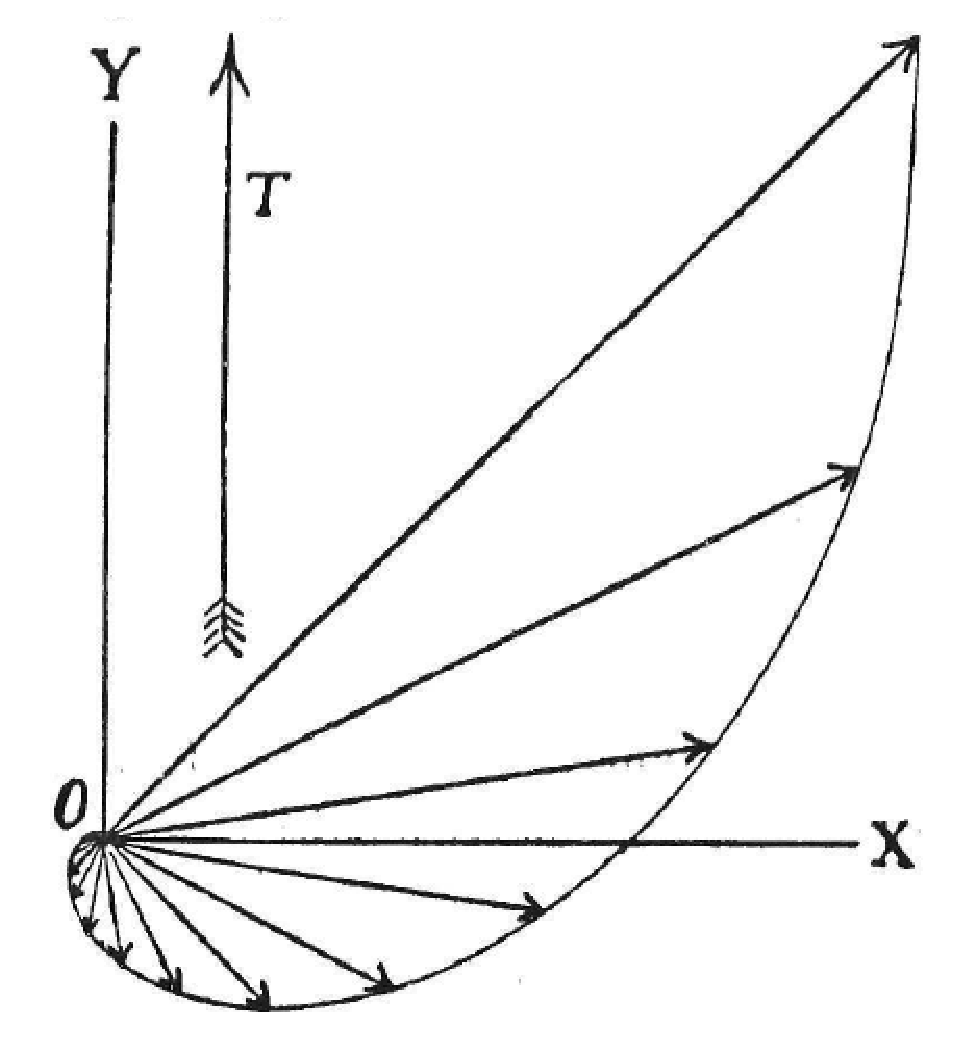
\includegraphics[width=5cm]{Ekman.eps}
		\caption*{} 
	\end{figure}
	\paragraph{水平体积输运}~{}\\
	体积输运:
	\[
	\begin{aligned}
	S &= \int_0^\infty  W dz \\
	&= {{{\tau _y}} \over {\sqrt 2 a\rho {A_z}}}{e^{i{\pi  \over 4}}}\int_0^\infty  {{e^{ - {\pi  \over {{D_0}}}(1 + i)z}}} dz\\
	&= {{{\tau _y}} \over {\sqrt 2 a\rho {A_z}}}{e^{i{\pi  \over 4}}}\left[ { - {{{D_0}} \over \pi }{1 \over {(1 + i)}}} \right]\left. {{e^{ - {\pi  \over {{D_0}}}(1 + i)z}}} \right|_0^\infty\\
	&= {{{\tau _y}} \over {2\Omega \sin \varphi \rho }} = {{{\tau _y}} \over {f\rho }}
	\end{aligned}
	\]
	\indent
    可以发现,得到的输运结果只有实部,没有虚部,说明体积输运方向为$x$轴正向,即在北半球水体向风向右侧90$\degree$输运.
    \subsubsection{有限深海漂流}
    \paragraph{假定}~{} \\
	有限深海Ekman漂流中用到了以下假定:\\
	\indent
	1) 海区无限广阔、有限深,远离海岸.\\
	\indent
	即无侧边界效应,仅有垂直湍流所生水平湍流摩擦力,并假定垂直湍流粘滞系数$A_z$为常量.由于海洋有限深,$z\rightarrow h,\vec{V}=0$\\
	\indent
	2) 定常均匀风场长时间作用.\\
	\indent
	即运动的基本参量与时间和水平坐标无关且海面无升降、无水平压强梯度.\\
	\indent
	3) 密度分布均匀,$\rho$为常数,不考虑热盐性质.\\
	\indent
    4) 采用$f$平面近似.\\
    控制方程和边界条件:
    \[
        \left\{
        \begin{aligned}
            &0=f v+A_{z} \frac{\partial^{2} u}{\partial z^{2}} \\
            &0=-f u+A_{z} \frac{\partial^{2} v}{\partial z^{2}}\\
            &\frac{\partial u}{\partial x}+\frac{\partial v}{\partial y}+\frac{\partial w}{\partial z}=0\\
            &z=0: \rho A_z\frac{\partial u}{\partial z}=0,\rho A_z\frac{\partial v}{\partial z}=-\tau_y\\
            &z\rightarrow h:u=v=0
        \end{aligned}
        \right.
    \]
    \paragraph{方程求解}~{}
    令$\xi=h-z$,定解问题化为:
    \begin{numcases}{}
        -fv=A_z\frac{\partial^2 u}{\partial \xi^2}\\
        fu=A_z\frac{\partial^2 v}{\partial \xi^2}\\
        \xi=h:\rho A_z\frac{\partial u}{\partial \xi}=0,\rho A_z\frac{\partial v}{\partial \xi}=\tau_y \nonumber\\
        \xi\rightarrow 0:u=v=0\nonumber
    \end{numcases}
    令$W=u+iv,\tau=\tau_x+i\tau_y$,控制方程:
    \[
        (11)+(12)\times i\Leftrightarrow \frac{d^{2} W}{d \xi^{2}}-j^{2} W=0
    \]
    边界条件:
    \[
        \begin{aligned}
            &\xi=h:\rho A_z\frac{\partial W}{\partial \xi}=\tau\\
            &\xi=0:W=0
        \end{aligned}
    \]
    与无限深海漂流解法类似,解得:
    \[
        W=\frac{(1+i) \tau_{y}}{2 a \rho A_{z}} \frac{s h(1+i) a \xi}{c h(1+i) a h}
    \]
    \paragraph{物理性质}~{}
    \paragraph{与水深的关系}~{}\\
    (1) $h≥2D_0$时,有限深海漂流流速流向与无限深海相同;
    (2) 水深越浅,流向随深度增加右偏(北半球)越缓慢;
    (3) 从上层到下层的流速矢量越是趋近风矢量的方向.
    \paragraph{体积输运}~{}\\
    (1) 在$x,y$方向(平行和垂直风向)都有输送;\\
    (2) 运输方向为风向右端,±90°之间:\\
        $$\displaystyle S_x>0;\\0<h<D_0,ah<\pi,S_y>0;D_0<h<2D_0,\pi<ah<2\pi,S_y<0;h>2D_0,S_y=0$$
    \subsubsection{漂流分离}
    \paragraph{利用风速大小相等、方向相反的两次观测余流分离漂流}~{}\\
    $\divideontimes$余流=漂流+恒量常流
    \begin{figure}[H]
        \centering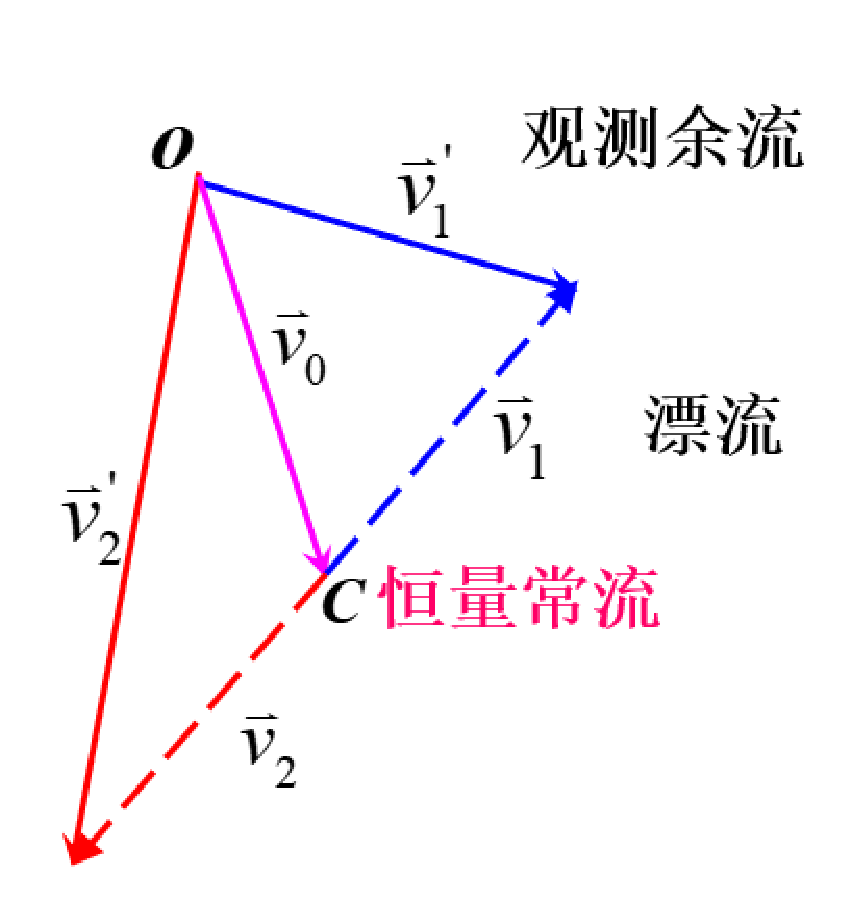
\includegraphics[width=5cm]{4.eps}
        \caption*{}
    \end{figure}
    \paragraph{利用一组风速大小相等、方向不同的实测余流分离漂流}~{}\\
    $\divideontimes$漂流速度矢量端点落在同一圆周上
    \begin{figure}[H]
        \centering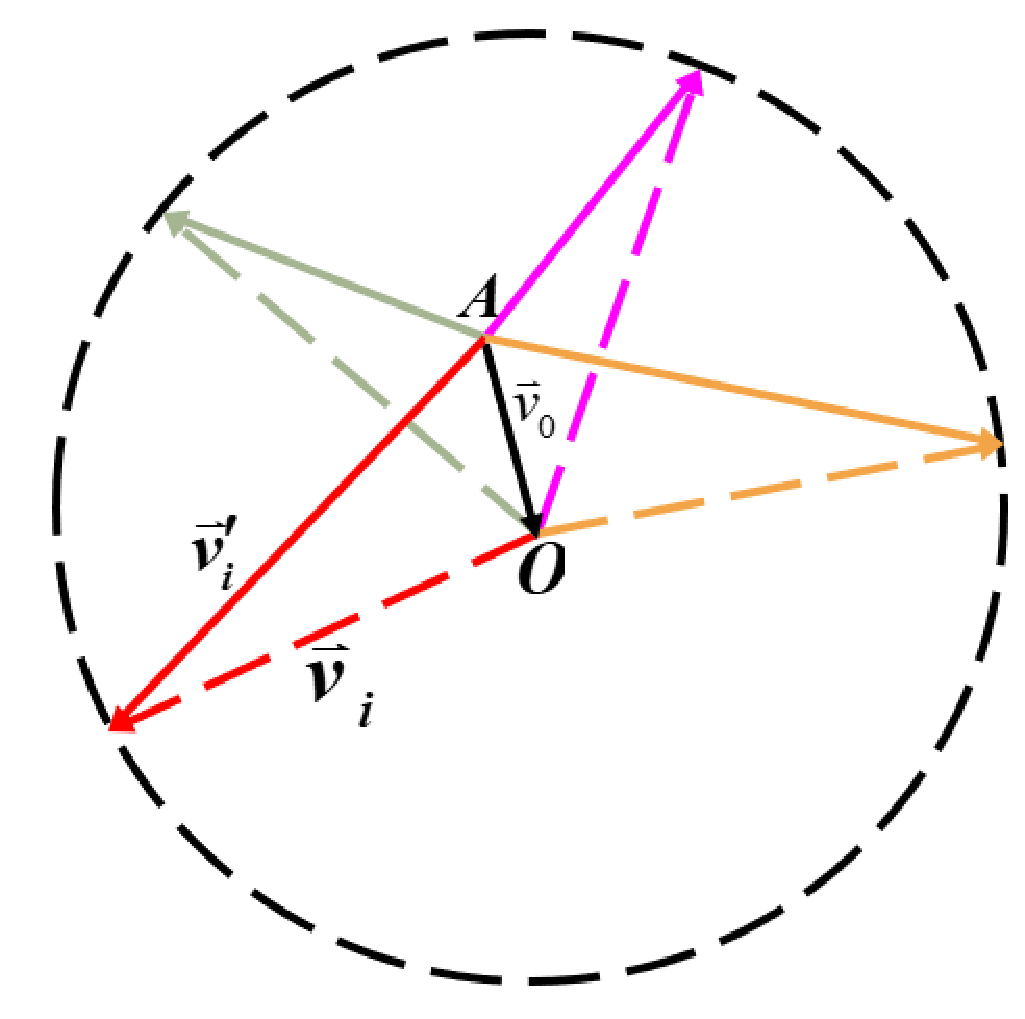
\includegraphics[width=5cm]{5.eps}
        \caption*{}
    \end{figure}
    \subsubsection{升降流}
    由不均匀风场或风场和地形配合产生的“较强烈”的铅直向流动。
    \paragraph{物理背景}~{}\\
    $\boxed{\mbox{非均匀风场}}\Rightarrow\boxed{\mbox{非均匀Ekman漂流}}\Rightarrow\boxed{\mbox{非均匀体积输运}}\Rightarrow\boxed{\mbox{辐聚辐散}}\mathop{\Rightarrow}\limits^{连续性}\boxed{\mbox{升降流}}$
    \begin{figure}[H]
        \centering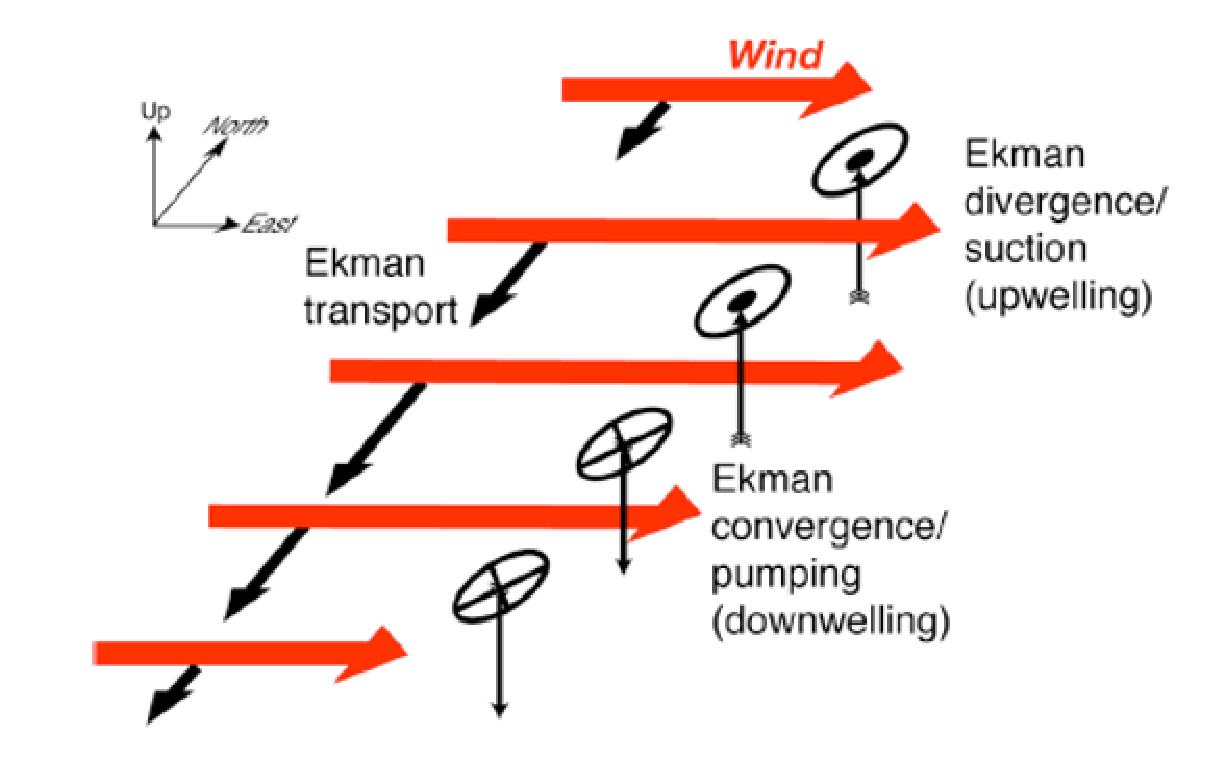
\includegraphics[width=8cm]{6.eps}
        \caption*{}
    \end{figure}
    \paragraph{赤道附近的升降流}~{} \\
    \begin{figure}[H]
        \centering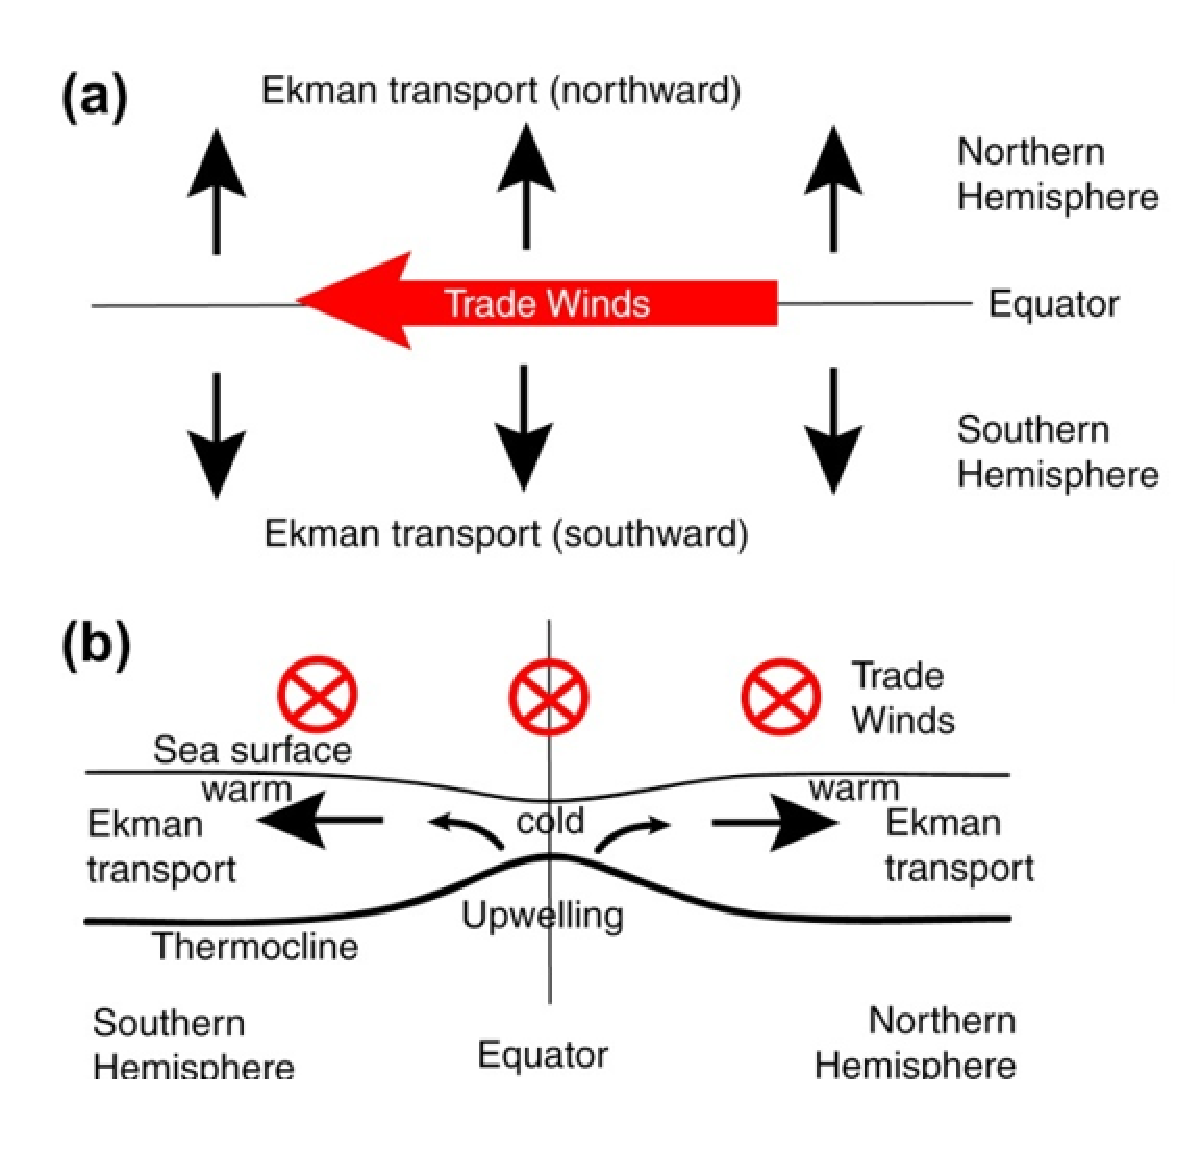
\includegraphics[width=8cm]{7.eps}
        \caption*{}
    \end{figure}
    \paragraph{顺(沿)岸风产生的升降流}~{} \\
    \begin{figure}[H]
        \centering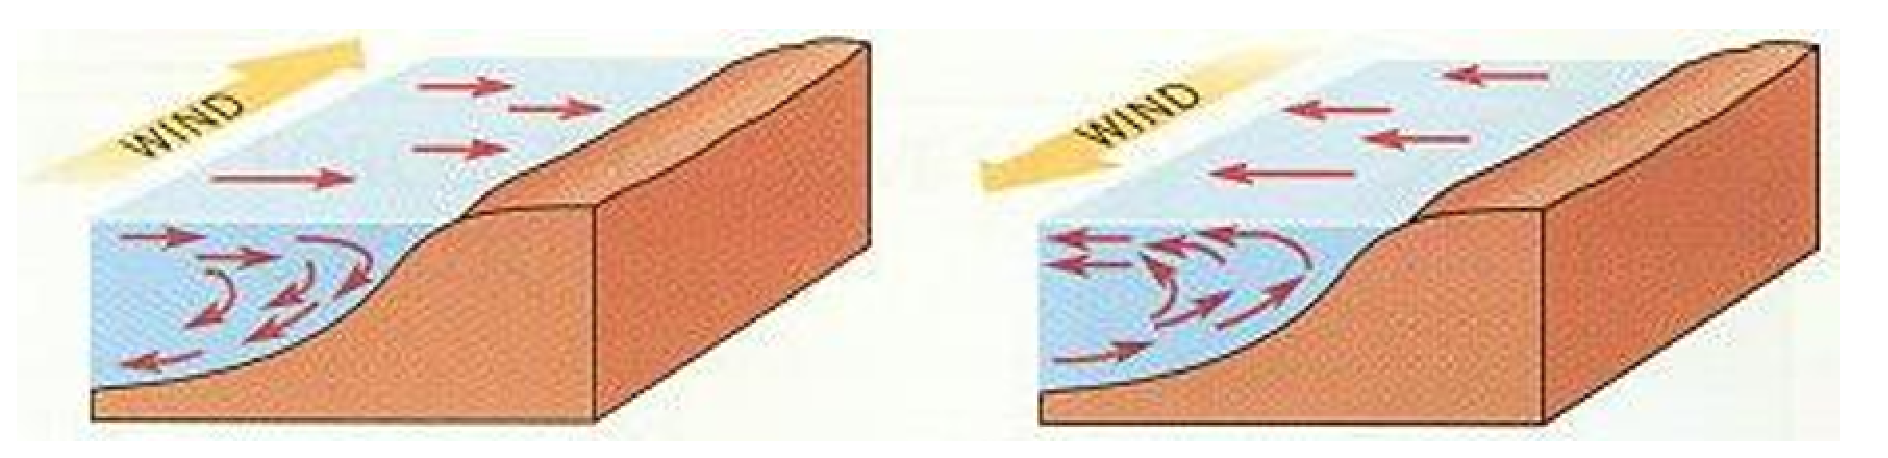
\includegraphics[width=10cm]{8.eps}
        \caption*{}
    \end{figure}
    \paragraph{气旋和反气旋产生的海洋升降流}~{} \\
    \begin{figure}[H]
        \centering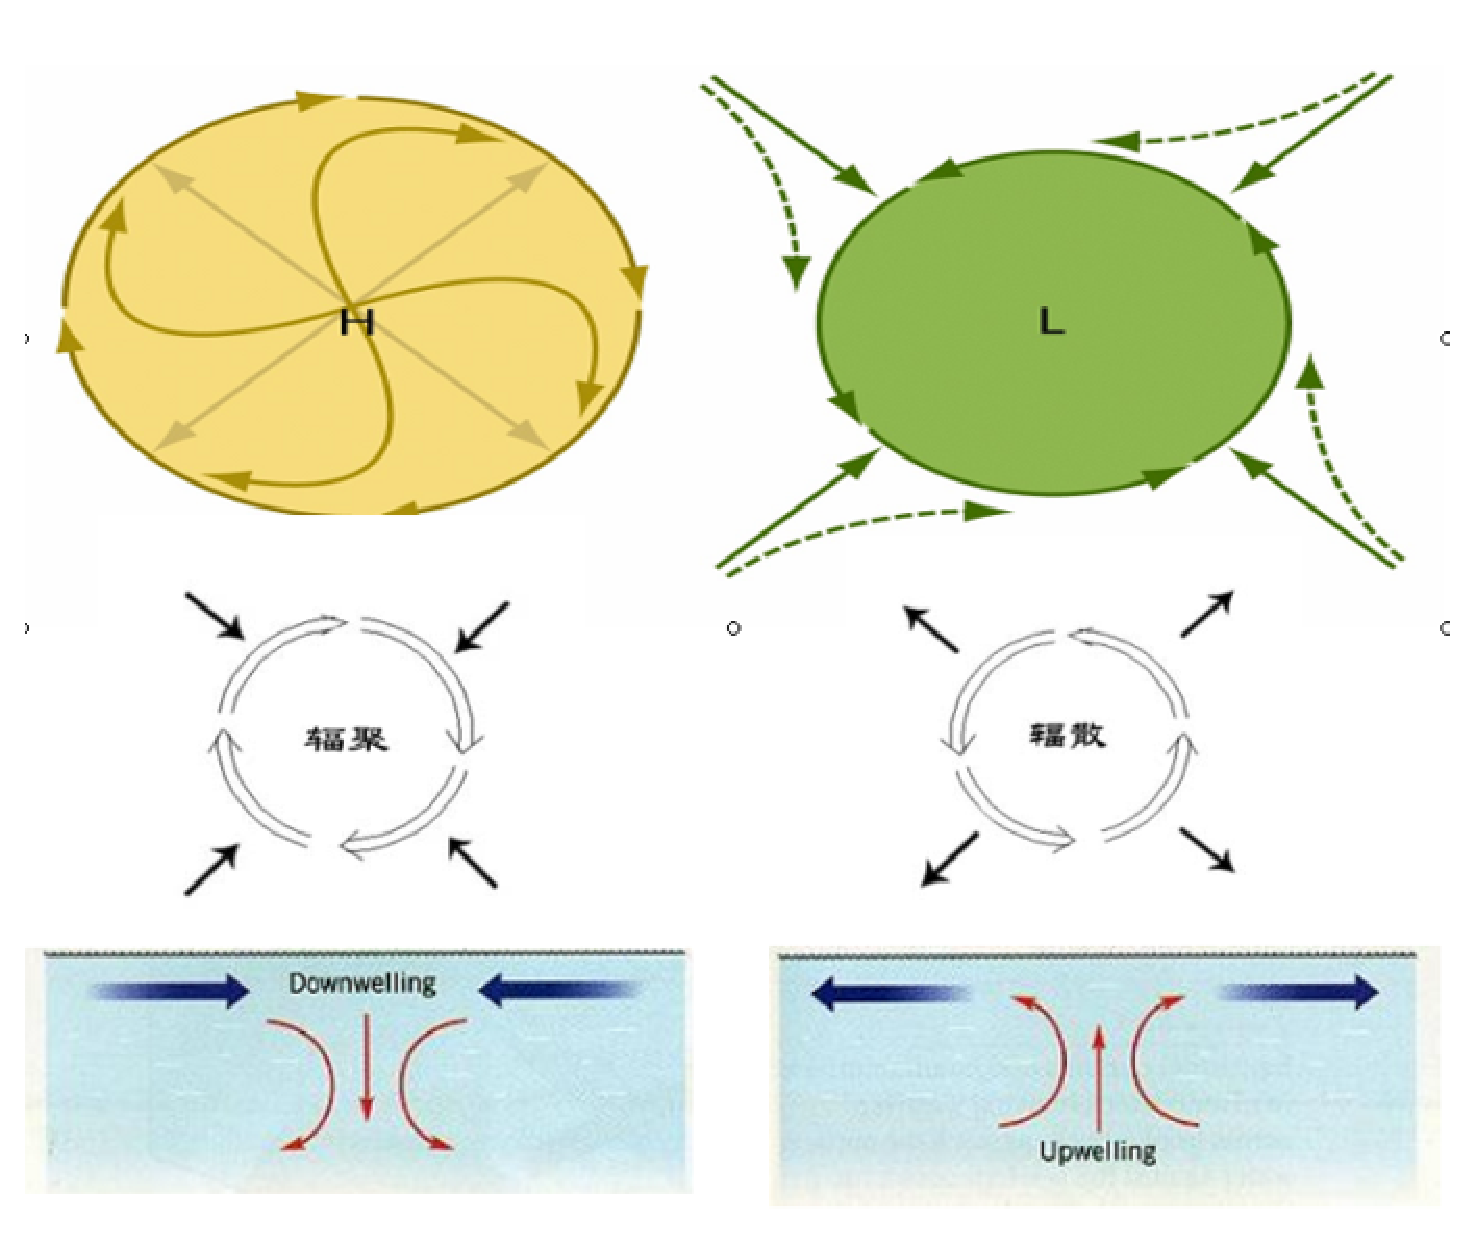
\includegraphics[width=8cm]{9.eps}
        \caption*{}
    \end{figure}
    \paragraph{假定}~{}\\
    (1) $\rho$为常数;\\
    (2) 直线风系,风仅沿$x$方向有变化;风区内为恒定的均匀风场;风区外无风;$\displaystyle \frac{\partial }{\partial y}=0$\\
    (3) 定常风场;$\displaystyle \frac{\partial }{\partial t}=0$\\
    (4) 大尺度;$Ro\ll 1$\\
    (5) 有限深度.$h \geq 2D_0$
    \paragraph{控制方程及边界条件}~{}
    \[
        \left\{
        \begin{aligned}
            &A_{l} \frac{\partial^{2} u}{\partial x^{2}}+A_{z} \frac{\partial^{2} u}{\partial z^{2}}+f v+g \frac{\partial \zeta}{\partial x}=0\\
            &A_{l} \frac{\partial^{2} v}{\partial x^{2}}+A_{z} \frac{\partial^{2} v}{\partial z^{2}}-f u=0\\
            &\frac{\partial u}{\partial x}+\frac{\partial w}{\partial z}=0
        \end{aligned}
        \right.
    \]
    \[
        \left\{
        \begin{aligned}
            &z=\zeta:\rho A_{z} \frac{\partial u}{\partial z}=0, \quad \rho A_{z} \frac{\partial v}{\partial z}=-\tau_{y} \quad(0 \leq x \leq L)\\
            &z=h:u=v=0\\
            &x=0:u=v=0\\
            &x\rightarrow\infty:u=v=0,\frac{\partial \zeta}{\partial x}=0
        \end{aligned}
        \right.
    \]
    \paragraph{结果讨论}~{}
    \begin{figure}[H]
        \centering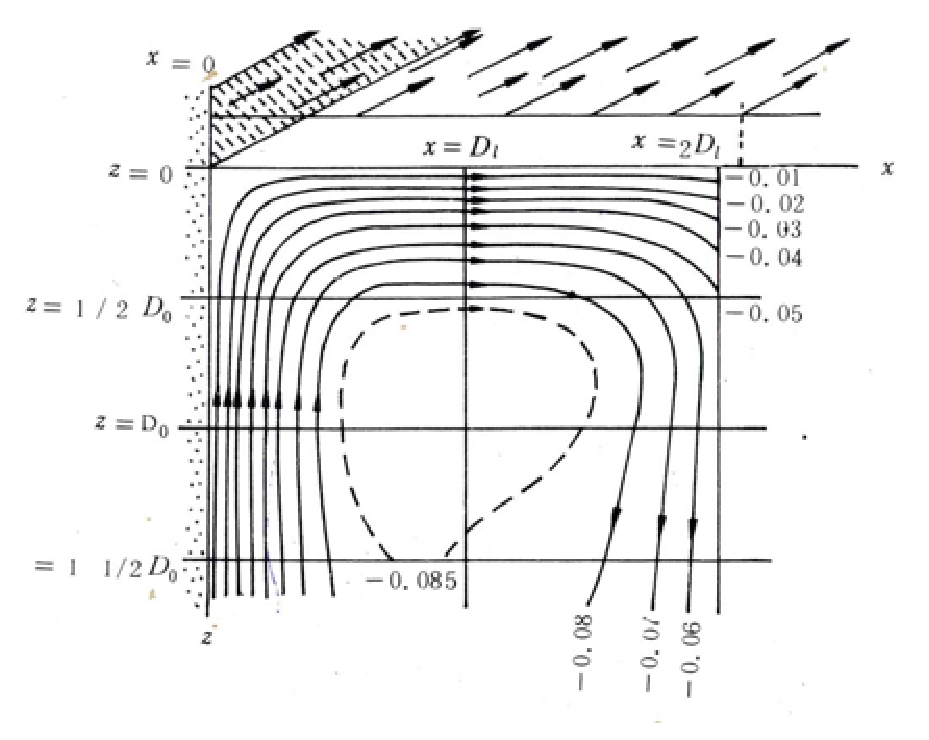
\includegraphics[width=8cm]{10.eps}
        \caption*{}
    \end{figure}
    (1) 近岸产生上升流$x\leq 0.5D_l$;\\
    (2) 风区外延附近下降流$x=2D_l$;\\
    (3) 上升流来自 $z=1.5D_0$或更深;\\
    (4) 最大$w$出现在$z=D_0$;\\
    (5) 上层离岸流,下层向岸流,构成一个循环.\\
    若风向与海岸成$\theta$角:\\
    \begin{figure}[H]
        \centering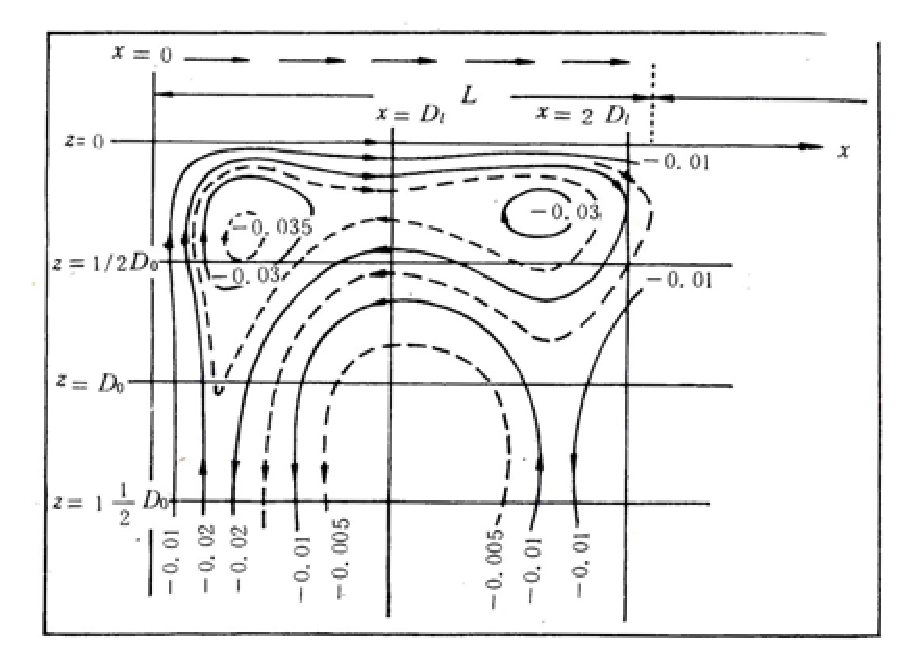
\includegraphics[width=8cm]{11.eps}
        \caption*{}
    \end{figure}
    (1) 三个升降流系统:两个顺时针,一个逆时针;\\
    (2) 大顺时针循环;\\
    (3) $\theta=21.5°$时,升降流达最大强度;\\
    (4) 纬度越低,升降流越强.
    \subsection{非定常运动}
    \subsubsection{漂流的发展}
    \paragraph{假定}~{} \\
    (1) 远离海岸和海底的开阔大洋;\\
    (2) 风场均匀恒定;\\
    (3) $\rho$为常数;\\
    (4) 海面无倾斜;\\
    (5) 运动非定常.\\
    \paragraph{控制方程}~{}
    \[
        \left\{
        \begin{aligned}
            &\frac{\partial u}{\partial t}-f v=A_{z} \frac{\partial^{2} u}{\partial z^{2}}\\
            &\frac{\partial v}{\partial t}+f u=A_{z} \frac{\partial^{2} v}{\partial z^{2}}
        \end{aligned}
        \right.
    \]
    \paragraph{初边值条件}~{}
    \[
        \left\{
        \begin{aligned}
            &z=0:A_z\frac{\partial u}{\partial z}=0,\rho A_z\frac{\partial v}{\partial z}=-\tau_y(t>0)\\
            &z\rightarrow\infty:u=v=0\\
            &t=0:u=v=0/u=C_1,v=C_2
        \end{aligned}
        \right.
    \]
    \paragraph{解的讨论}~{}
    \[
        \left\{
        \begin{aligned}
            &u=\frac{2 \pi \tau_{y}}{\rho f D_{0}} \int_{0}^{t^{\prime}} \frac{\sin (2 \pi \eta)}{\sqrt{\eta}} e^{\frac{\pi z^2}{4 D_{0}^{2}}} d \eta \\
            &v=\frac{2 \pi \tau_{y}}{\rho f D_{0}} \int_{0}^{t^{\prime}} \frac{\cos (2 \pi \eta)}{\sqrt{\eta}} e^{\frac{\pi z^2}{4 D_{0}^{2}}} d \eta
        \end{aligned}
        \right.
    \]
    根据下图\cite{Ekman}:
    \begin{figure}[H]
        \centering 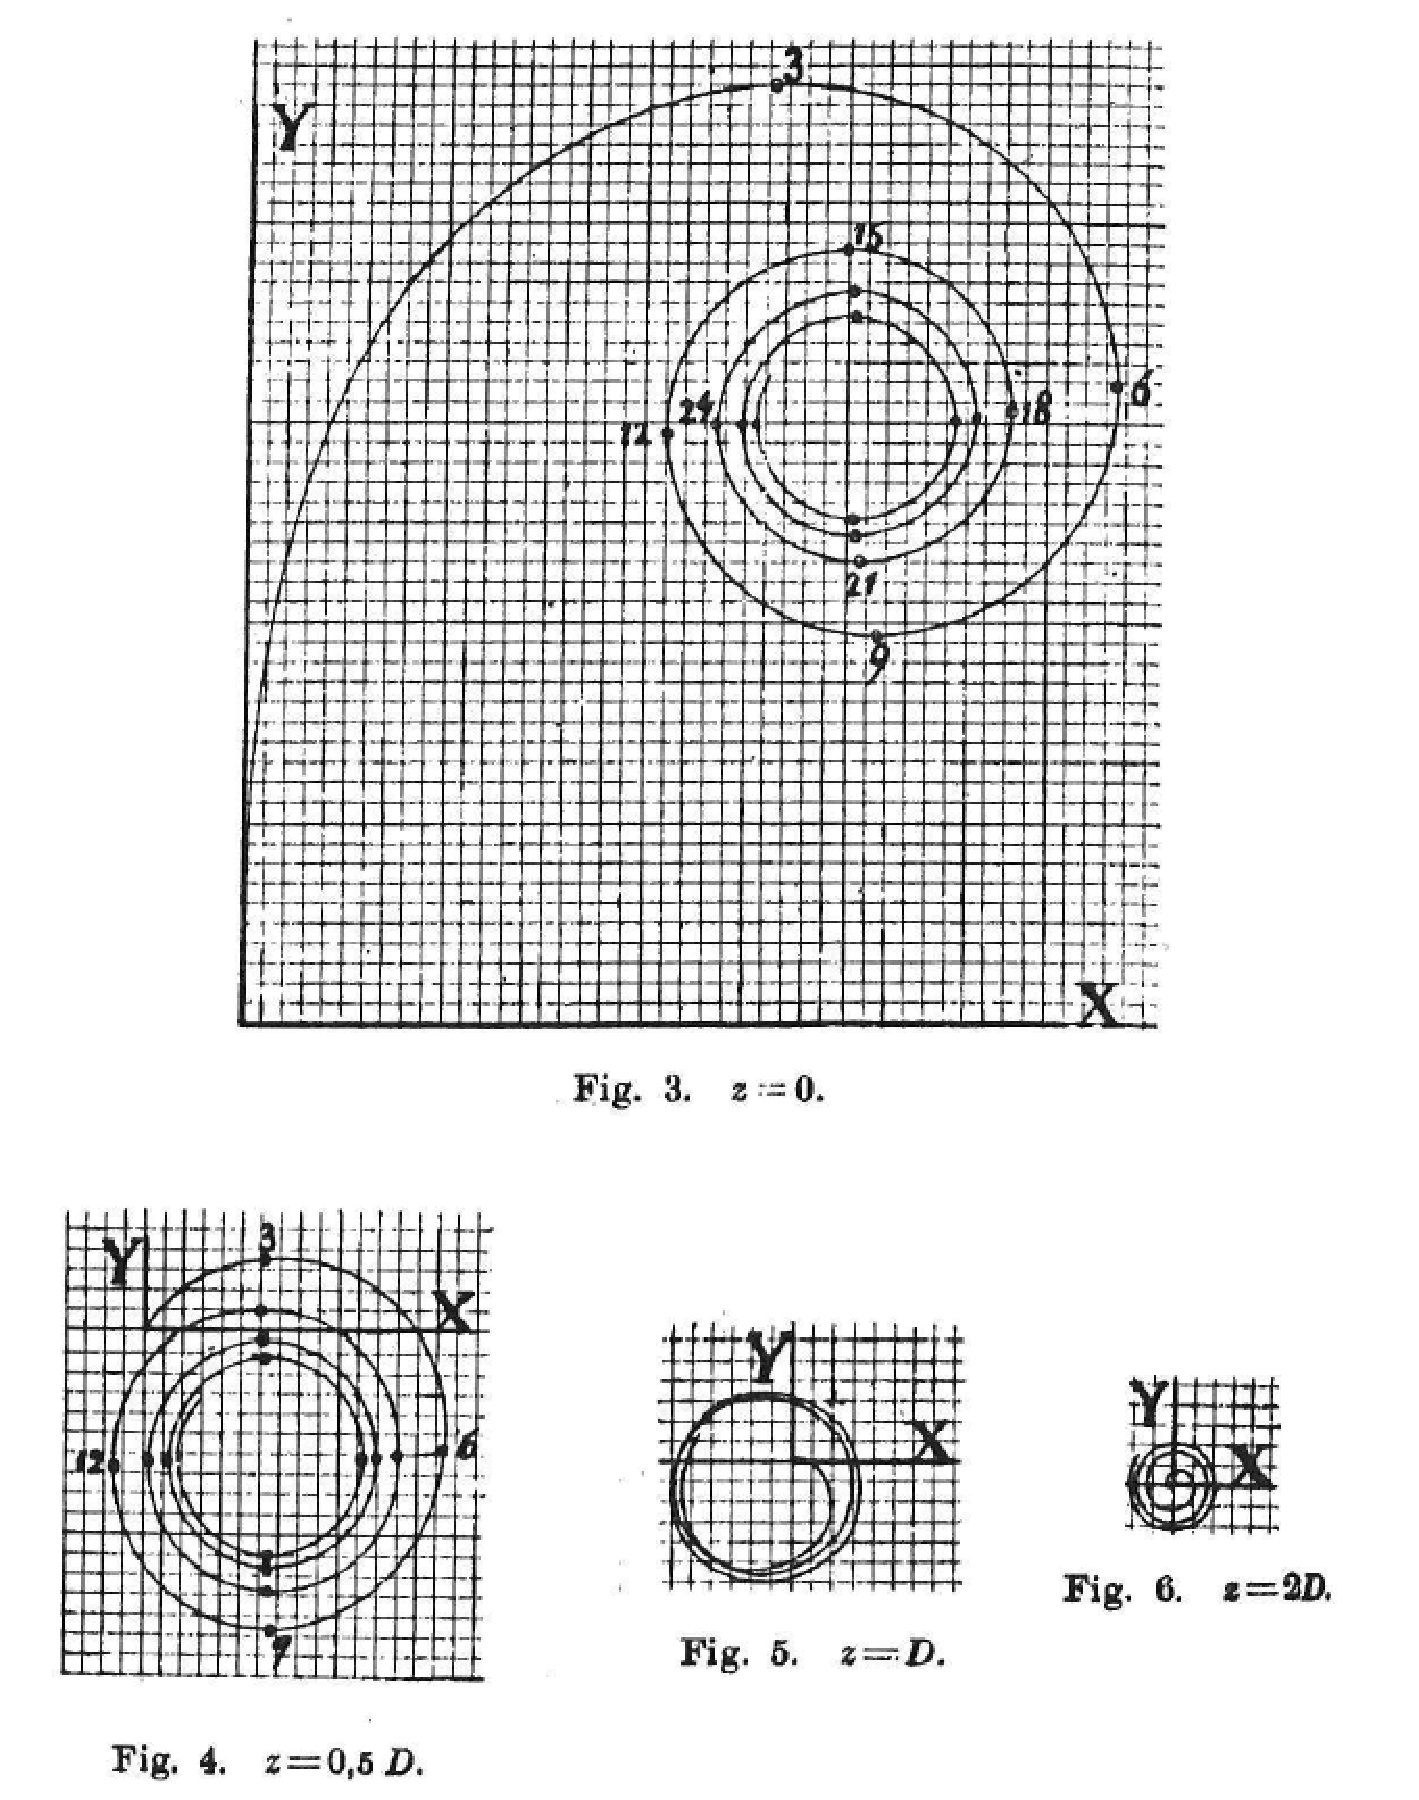
\includegraphics[width=7cm]{12.eps}
        \caption*{}
    \end{figure}
    随时间增加,空间某点流苏端点顺时针旋转(北半球),逐渐趋向一个极限值(即漂流).
    \subsubsection{惯性流}
    \paragraph{假定和方程}~{} \\
    (1) 风场消失或者流动离开风区;\\
    (2) 外部驱动小时,湍摩擦失去作用;\\
    (3) 流动转为由惯性项维持平衡;\\
    (4) 强制流动转变为自由流动.\\
    \begin{numcases}{}
        \frac{du}{dt}-fv=0 \label{ic1}\\
        \frac{dv}{dt}+fu=0 \label{ic2}
    \end{numcases}
    \paragraph{求解}~{}
    \[
        \begin{aligned}
            (\ref{ic1})\times u+(\ref{ic2}\times v)&\Leftrightarrow u \frac{d u}{d t}+v \frac{d v}{d t}=\frac{1}{2} \frac{d u^{2}}{d t}+\frac{1}{2} \frac{d v^{2}}{d t}=0 \\
            &\Leftrightarrow \frac{d}{d t}\left(u^{2}+v^{2}\right)=0\\
            &\Leftrightarrow u^{2}+v^{2}=c=V_{0}^{2}
        \end{aligned}
    \]
    \[
        \begin{aligned}
            (\ref{ic1}),(\ref{ic2})
            &\Rightarrow
            \left\{\begin{aligned}&v=\frac{d y}{d t}=\frac{1}{f} \frac{d u}{d t}\\ &u=\frac{d x}{d t}=\frac{1}{f} \frac{d v}{d t}\end{aligned}\right.\\
            &\Rightarrow
            \left\{\begin{aligned}&y-y^{\prime}=\frac{1}{f}\left(u-u^{\prime}\right)\\ &x-x^{\prime}=-\frac{1}{f}\left(v-v^{\prime}\right)\end{aligned}\right.\\
            &\Rightarrow
            \left\{\begin{aligned}&y-\left(y^{\prime}-\frac{u^{\prime}}{f}\right)=\frac{u}{f}\\ &x-\left(x^{\prime}+\frac{v^{\prime}}{f}\right)=-\frac{v}{f}\end{aligned}\right.\\
            &\Rightarrow\boxed{\left(y-y_{0}\right)^{2}+\left(x-x_{0}\right)^{2}=\frac{1}{f^{2}}\left(u^{2}+v^{2}\right)=\frac{V^{2}}{f^{2}}=r^{2}}
        \end{aligned}
    \]
    流体质点沿半径为$r$的圆周作匀速运动,这个圆称之为惯性圆,对应的流动为惯性流.
    \paragraph{惯性圆半径}~{}\\
    科氏力充当向心力:$\displaystyle \frac{V_0^2}{r}=fV_0\Rightarrow V_0=fr\Rightarrow r=\frac{V_0}{f}=\frac{V_0}{2\omega \sin \varphi}$\\
    随纬度增加而减小;赤道$r\rightarrow\infty$,水质点作直线运动.
    \paragraph{周期}~{}
     \[
        T_{i}=\frac{2 \pi r}{V_{0}}=\frac{2 \pi r}{f r}=\frac{2 \pi}{f}=\frac{\pi}{\omega \sin \varphi}
     \]
     \paragraph{运动方向}~{}\\
     北半球,顺时针;南半球,逆时针.
    \paragraph{背景流}~{}\\
    (1) 当无其他外加流动时,所有惯性圆的圆心位于同一条铅直线上,因而海水就像以角速度$2\omega \sin \varphi$旋转的刚体一样;\\
    (2) 当有其他外加流动时,除了在同一水平面上所有海水质点皆在同一时刻由同一流速速率外,还依外加流动速度方向移动.
    \newpage
    \subsection{风生大洋环流}
    \subsubsection{Sverdrup理论}
    \paragraph{假定}~{}\\
    (1) 远离海岸的大洋中部海区,Ro$\ll 1$大尺度、等深大洋$h$为常数;\\
    (2) 远离边界、无侧边界影响,无水平湍摩擦应力E$_l\ll 1$;\\
    (3) 定常风 定常流动;\\
    (4) $\rho$为常数;\\
    (5) $\beta$平面近似.\\
    \paragraph{控制方程}~{}
    \[
        \left\{
            \begin{aligned}
                &-f v=-\frac{1}{\rho} \frac{\partial p}{\partial x}+A_{z} \frac{\partial^{2} u}{\partial^{2} z} \\
                &fu=-\frac{1}{\rho} \frac{\partial p}{\partial y}+A_{z} \frac{\partial^{2} v}{\partial^{2} z} \\
                &0=-\frac{1}{\rho} \frac{\partial p}{\partial z}-g\\
                &\frac{\partial u}{\partial x}+\frac{\partial v}{\partial y}+\frac{\partial w}{\partial z}=0
            \end{aligned}
        \right.
    \]
    \paragraph{边界条件}~{}
    \[
        \left\{
            \begin{aligned}
                &z=\zeta(\mbox{海面}):\rho A_z\frac{\partial u}{\partial z}=\tau_{x\zeta},\rho A_z\frac{\partial v}{\partial z}=\tau_{y\zeta}\\
                &z=-h(\mbox{足够深}):u=v=0,\frac{\partial u}{\partial z}=\frac{\partial v}{\partial z}=0,\frac{\partial p}{\partial x} =\frac{\partial p}{\partial y}=0
            \end{aligned}
        \right.
    \]
    \paragraph{求解}~{}\\
    对上式进行垂直积分:
    \begin{numcases}{}
        -fM_y=-\frac{\partial P}{\partial x}+\tau_{x\zeta}\\
        fM_x=-\frac{\partial P}{\partial y}+\tau_{y\zeta}\\
        \frac{\partial M_x}{\partial x}+\frac{\partial M_y}{\partial y}=0\nonumber
    \end{numcases}
    其中,$\displaystyle M_x=\int_{-h}^0\rho udz,M_y=\int_{-h}^0\rho vdz,P=\int_{-h}^0 pdz,\tau_{x\zeta}=\int_{-h}^0\rho A_z\frac{\partial^2 u}{\partial z^2}=\rho A_{z}\left(\left.\frac{\partial u}{\partial z}\right|_{z=0}-\left.\frac{\partial u}{\partial z}\right|_{z=-h}\right)\quad (\zeta\ll h)$
    \[
        \begin{aligned}
            \frac{\partial (1)}{\partial y}-\frac{\partial (2)}{\partial x}&\Leftrightarrow -M_y\frac{\partial f}{\partial y}\mathop{\boxed{-f\frac{\partial M_y}{\partial y}-f\frac{\partial M_x}{\partial x}}}\limits^{0}=\frac{\partial \tau_{x\zeta}}{\partial y}-\frac{\partial \tau_{y\zeta}}{\partial x}\\
            &\Leftrightarrow M_{y} \frac{\partial f}{\partial y}=\frac{\partial \tau_{y \zeta}}{\partial x}-\frac{\partial \tau_{x \zeta}}{\partial y}\\
            &\Leftrightarrow\mathop{\boxed{\color{red}\beta M_y=\operatorname{rot}_z\tau_\zeta}}\limits_{\mbox{Sverdrup方程}}
        \end{aligned}
    \]
    $\color{red} \mbox{Sverdrup方程的物理意义1}$:海水南北向的输运由风应力旋度所驱动.
    \paragraph{讨论}~{}\\
    将质量输运分为Ekman漂流输运与地转流输运两部分:
    \[
        \begin{aligned}
            &M_x=M_{xE}(\mbox{Ekman漂流})+M_{xg}(\mbox{地转流})\\
            &M_y=M_{yE}(\mbox{Ekman漂流})+M_{yg}(\mbox{地转流})
        \end{aligned}
    \]
    \begin{numcases}{}
        -fM_{yE}=\tau_{x\zeta}\\
        fM_{xE}=\tau_{y\zeta}\\
        -fM_{yg}=-\frac{\partial P}{\partial x}\\
        fM_{yg}=-\frac{\partial P}{\partial y}
    \end{numcases}
    \begin{align}
        &\frac{\partial(17)}{\partial y}-\frac{\partial(18)}{\partial x}\Leftrightarrow\frac{\partial {M}_{xE}}{\partial x}+\frac{\partial {M}_{yE}}{\partial y}=\boxed{\nabla \cdot \vec{{M}}_{E}=\left(\operatorname{rot}_{z} \vec{\tau}_{\zeta}-{\beta} {M}_{y E}\right) / {f}}\\
        &\frac{\partial(19)}{\partial y}-\frac{\partial(20)}{\partial x}\Leftrightarrow\frac{\partial {M}_{xg}}{\partial x}+\frac{\partial {M}_{yg}}{\partial y}=\boxed{\nabla \cdot \vec{{M}}_{g}=-\beta M_{yg}/f}
    \end{align}
    (1) Ekman漂流质量输运的水平散度与$\circled{1}$风应力旋度$\circled{2} f\circled{3} \beta$有关.\\
    (2) 地转流质量输运的水平辐散引起南北向的地转运动.
    \[
        (21)+(22)\Leftrightarrow \operatorname{rot}_z\vec{tau}_\zeta-\beta M_y=0\Leftrightarrow\boxed{\color{red} \beta M_y=\operatorname{rot}_z\vec{\tau}_\zeta}
    \]
    $\color{red} \mbox{Sverdrup方程的物理意义2}$:地转流流量的散度和Ekman漂流流量的散度相平衡,所以Sverdrup方程又称Sverdrup平衡.\\
    (1) 所有南北向的地转运动,必须显示水平散度;\\
    (2) 虽然Ekman漂流流量的散度与地转流流量的散度本身不为0,但是它们的和,即总流量的水平散度必须为0,说明Ekman漂流流量的散度和地转流流量的散度刚好取得平衡;\\
    (3) $\operatorname{rot}_z\vec{\tau}_\zeta=0$:只存在东西方向的输运,$\operatorname{rot}_z\vec{\tau}_\zeta>0$:质量输运向北(北半球),$\operatorname{rot}_z\vec{\tau}_\zeta<0$:质量输运向南(南半球);\\
    (4) 地转流引起的南北质量运输量比Ekman漂流引起的大.
    \paragraph{缺陷}~{}\\
    设仅有纬向风,且$\tau_{x\zeta}$仅为$y$的函数:
    \[
        M_y=\frac{1}{\beta}\operatorname{rot}_z\vec{\tau}_\zeta=\frac{1}{\beta}\left(\cancel{\frac{\partial \tau_{y\zeta}}{\partial x}}-\frac{\partial \tau_{x\zeta}}{\partial y}\right)=-\frac{a}{2\omega\cos\varphi}\frac{\partial\tau_{x\zeta}}{\partial y}
    \]
    \[
        \frac{\partial M_{x}}{\partial x}=-\frac{\partial M_{y}}{\partial y}\Rightarrow M_{x}=\frac{x}{2 \omega \cos \varphi}\left(a \frac{\partial^{2} \tau_{x f}}{\partial y^{2}}+\frac{\partial \tau_{x f}}{\partial y} t g \varphi\right)+{\color{red}c(y)}
    \]
    在东、西边界,$M_x=0$而Sverdrup理论不能同时满足.
    \subsubsection{Stommel理论}
    \paragraph{假定}~{}\\
    (1) 远离海岸的大洋中部海区,Ro$\ll 1$大尺度、等深大洋$h$为常数;\\
    (2) 远离边界、无侧边界影响,无水平湍摩擦应力E$_l\ll 1$;\\
    (3) 定常风 定常流动;\\
    (4) $\rho$为常数;\\
    (5) $\beta$平面近似;\\
    $\mbox{(6) 考虑底摩擦}$
    \paragraph{控制方程}~{}
    \[
        \left\{
            \begin{aligned}
                &-f v=-g \frac{\partial \zeta}{\partial x}+A_{z} \frac{\partial^{2} u}{\partial^{2} z} \\
                &fu=-g \frac{\partial \zeta}{\partial y}+A_{z} \frac{\partial^{2} v}{\partial^{2} z} \\
                &0=-\frac{1}{\rho} \frac{\partial p}{\partial z}-g\\
                &\frac{\partial u}{\partial x}+\frac{\partial v}{\partial y}+\frac{\partial w}{\partial z}=0
            \end{aligned}
        \right.
    \]
    \paragraph{边界条件}~{}
    \[
        \left\{
            \begin{aligned}
                &z=\zeta(\mbox{海面}):\tau_{x , \zeta}=\left.\rho A_{z} \frac{\partial u}{\partial z}\right|_{t=\zeta}=-F \cos (\pi y / b),\tau_{x , \zeta}=0\\
                &z=-h(\mbox{海底}):\tau_{x,-h}=\rho+\left.\frac{\partial u}{\partial z}\right|_{t=-h}={\color{red}\rho k u},\tau_{y,-h}=\rho+\left.\frac{\partial v}{\partial z}\right|_{t=-h}={\color{red}\rho k v}
            \end{aligned}
        \right.
    \]
    \paragraph{求解}~{}\\
    对上式进行垂直平均:
    \[
        \left\{
        \begin{aligned}
            &-f\left\langle v\right\rangle=-g \frac{\partial \zeta}{\partial x}+\left.\frac{A_{z}}{h+\zeta} \frac{\partial u}{\partial z}\right|_{\zeta}-\left.\frac{A_z}{h+\zeta} \frac{\partial u}{\partial z}\right|_{-h}\\
            &f\left\langle u\right\rangle=-g \frac{\partial \zeta}{\partial y}+\left.\frac{A_{z}}{h+\zeta} \frac{\partial v}{\partial z}\right|_{\zeta}-\left.\frac{A_z}{h+\zeta} \frac{\partial v}{\partial z}\right|_{-h}\\
            &\frac{\partial}{\partial x}\left[\left(n+\zeta\right)\left\langle u\right\rangle\right]+\frac{\partial}{\partial y}[(n+\zeta)\left\langle v\right\rangle]=0
        \end{aligned}
        \right.
    \]
    
    将边界条件代入方程:
    \begin{numcases}{}
        0=f \rho h v-F \cos \left(\left. \pi y \middle/ b \right.\right)-\rho k u-\rho g h \frac{\partial \zeta}{\partial x} \quad(\zeta \ll k) \label{stm1}\\
        0=-f \rho h u-\rho k v-\rho g h \frac{\partial \zeta}{\partial y}\label{stm2}\\
        \frac{\partial u}{\partial x}+\frac{\partial v}{\partial y}=0 \nonumber
    \end{numcases}
    \[
        \frac{\partial (\ref{stm1})}{\partial y}-\frac{\partial (\ref{stm2})}{\partial x}\Rightarrow \frac{h}{k}[\beta v+r \sin (\pi y / b)]+{\color{red}\overbrace{\left(\frac{\partial v}{\partial x}-\frac{\partial u}{\partial y}\right)}^{\color{red}\mbox{来源于底摩擦}}}=0
    \]
    引入流函数$\displaystyle \psi:u=\frac{\partial \psi}{\partial y},v=-\frac{\partial \psi}{\partial x}$:
    \[
        {\color{red}\overbrace{\frac{\partial^{2} \psi}{\partial x^{2}}+\frac{\partial^{2} \psi}{\partial y^{2}}}^{\color{red}\mbox{来源于底摩擦}}}+\frac{h}{k} \beta \frac{\partial \psi}{\partial x}=\frac{h}{k} r \sin \frac{\pi y}{b}
    \]
    边界条件:
    \[
        \psi(0, y)=\psi(a, y)=\psi(x, 0)=\psi(x, b)=0
    \]
    \[
        \Rightarrow \psi(x, y)=\frac{F b}{k \pi} \sin \frac{\pi y}{b}\left[\frac{e^{\frac{h \beta}{2 k}(a-x)} \operatorname{sh} \alpha x+e^{\frac{h \beta}{2 k} x} \operatorname{sh} \alpha(a-x)}{\operatorname{sh} \alpha a}-1\right]
    \]
    特别地,若$\beta=0$:$\displaystyle\psi(x, y)=\frac{F b}{k \pi} \sin \frac{\pi y}{b}\left[\frac{\operatorname{sh} \frac{\pi}{b} x+\operatorname{sh} \frac{\pi}{b}(a-x)}{\operatorname{sh} \frac{\pi}{b} a}-1\right]$
    \paragraph{讨论}~{图片来自$Introduction \;to \; Physical \;Oceanography$(Robert H. Stewart,2008 pp190)}
    \begin{figure}[H]
        \centering 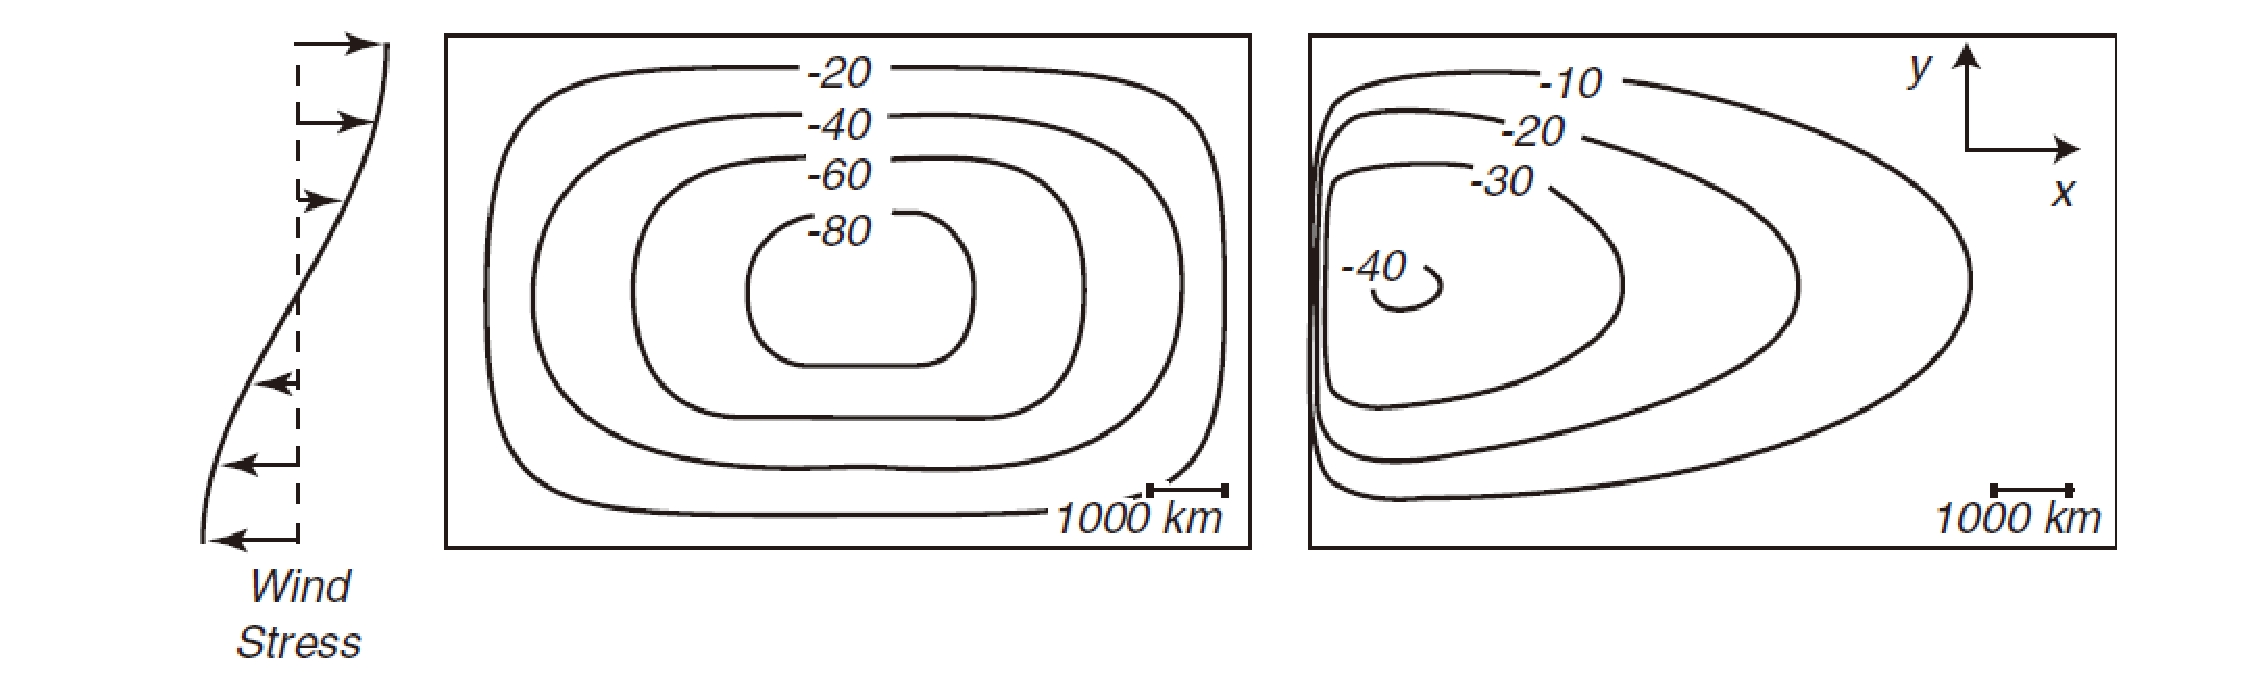
\includegraphics[width=18cm]{13.eps}
        \caption*{\large$  \color{red}\divideontimes\beta\mbox{效应导致了西向强化现象.}$}
    \end{figure}
    \begin{framed}
    \begin{multicols}{2}
        \begin{spacing}{0.8}
        \centering 
        $\mathbf\beta=0$(非旋转坐标系或f平面近似):\\
        (1) 流线南北对称;\\
        (2) 流线东西对称.\\
        $\mathbf\beta\neq 0$($\beta$平面近似):\\
        (1) 流线南北对称;\\
        (2) 流线东西不对称,西部密集,东部稀疏.
        \end{spacing}
    \end{multicols}
    \end{framed}
    \subsubsection{惯性理论}
    \paragraph{方程}~{}\\
    在Sverdrup理论的控制方程中引入惯性项:
    \[
        \left\{
            \begin{aligned}
                &\frac{du}{dt}-f v=-\frac{1}{\rho} \frac{\partial p}{\partial x}+A_{z} \frac{\partial^{2} u}{\partial^{2} z} \\
                &\frac{dv}{dt}+fu=-\frac{1}{\rho} \frac{\partial p}{\partial y}+A_{z} \frac{\partial^{2} v}{\partial^{2} z} \\
                &0=-\frac{1}{\rho} \frac{\partial p}{\partial z}-g\\
                &\frac{\partial u}{\partial x}+\frac{\partial v}{\partial y}+\frac{\partial w}{\partial z}=0
            \end{aligned}
        \right.
    \]
    \paragraph{求解}~{}
    \paragraph{内区(中部区)}~{}\\
    满足Sverdrup理论:$\displaystyle \beta M_y=\operatorname{rot}_z\tau_\zeta,M_y=\frac{\partial \varphi}{\partial x}=\frac{1}{\beta} \operatorname{rot}_{z} \tau_{\zeta}=\frac{1}{\beta}\left(\frac{\partial \tau_{y\zeta}}{\partial x}-\frac{\partial \tau_{x\zeta}}{\partial y}\right)$\\
    又设风应力:$\displaystyle \tau_{x\zeta}=-W\left(1-\frac{y^2}{s^2}\right),\tau_{y\zeta}=0\quad (0\leq y \leq s)$\\
    \[
        \begin{aligned}
            \Rightarrow &\frac{\partial \varphi}{\partial x}=-\frac{2W}{\beta s^2}y\\
            \Rightarrow &\varphi=-\frac{2W}{\beta s^2}yx+C(y)\\
            (x=r:\varphi=0)\quad &0=-\frac{2W}{\beta s^2}yr+C(y)\\
            \Rightarrow &\varphi=\frac{2W}{\beta s^2}y(r-x)
        \end{aligned}
    \]
    \paragraph{大洋西部海域}~{}\\
    不考虑湍摩擦效应:
    \begin{numcases}{}
        \frac{du}{dt}-f v=-\frac{1}{\rho} \frac{\partial p}{\partial x} \label{int1}\\
        \frac{dv}{dt}+fu=-\frac{1}{\rho} \frac{\partial p}{\partial y} \label{int2}\\
        0=-\frac{1}{\rho} \frac{\partial p}{\partial z}-g\nonumber\\
        \frac{\partial u}{\partial x}+\frac{\partial v}{\partial y}+\frac{\partial w}{\partial z}=0\nonumber
    \end{numcases}
    \begin{align}
            \frac{\partial (\ref{int2})}{\partial x}-\frac{\partial (\ref{int1})}{\partial y}           &\Leftrightarrow \frac{d}{d t}(\xi_r+f)+(\xi_r+f)\left(\frac{\partial u}{\partial x}+\frac{\partial v}{\partial y}\right)=0 \nonumber\\
            &\Leftrightarrow \frac{d}{d t}\left(\xi_{r}+f\right)=-\left(\xi_{r}+f\right)\left(\frac{\partial u}{\partial x}+\frac{\partial v}{\partial y}\right) \label{int3}
    \end{align}
    $\displaystyle \xi_r=\frac{\partial v}{\partial x}-\frac{\partial u}{\partial y}$相对涡度,$f$行星涡度,$\xi_a=\xi_r+f$绝对涡度.\\
    对连续方程进行垂向平均:
    \begin{align}
        &\frac{\partial \zeta}{\partial t}+\frac{\partial[(h+\zeta)\langle u\rangle]}{\partial x}+\frac{\partial[(h+\zeta)(v)]}{\partial y}=0\nonumber\\
        \Leftrightarrow & \frac{d(\zeta+h)}{d t}+(\zeta+h)\left(\frac{\partial(u)}{\partial x}+\frac{\partial(v)}{\partial y}\right)=0 \nonumber\\
        (\mbox{令}H=h+\zeta)\Leftrightarrow & \frac{d H}{d t}+H\left(\frac{\partial u}{\partial x}+\frac{\partial v}{\partial y}\right)=0 \label{int4}
    \end{align}
    将$(\ref{int4})$代入$(\ref{int3})$中:
    \begin{align}
         &\Rightarrow \frac{d}{d t}\left(\xi_{r}+f\right)=\frac{1}{H}\left(\xi_{r}+f\right) \frac{d H}{d t}\nonumber\\
         &\Rightarrow \frac{1}{H} \frac{d}{d t}(\xi_r+f)=\frac{1}{H^{2}}\left(\xi_{r}+f\right) \frac{d H}{d t}\nonumber\\
         &\Rightarrow {\color{red} \boxed{\frac{d}{d t}\left(\frac{\xi_{r}+f}{H}\right)=0}} \label{veq}
    \end{align}
    $(\ref{veq})$为$\color{red}\mbox{位势涡度守恒方程}$.\\
    假设在西边界区$\displaystyle\frac{\partial u}{\partial y}=0$,则:
    \[
        \xi_{r}=\frac{\partial v}{\partial x}-\frac{\partial u}{\partial y}=\frac{\partial v}{\partial x}=\frac{\partial}{\partial x}\left(\frac{1}{H} \frac{\partial \varphi}{\partial x}\right)
    \]
    代入$(\ref{veq})$:
    \[
        \begin{aligned}
            &\frac{d}{d t}\left[\frac{\frac{\partial}{\partial x}\left(\frac{1}{M} \frac{\partial \varphi}{\partial x}\right)+f}{H}\right]=0\\
            \Rightarrow & \frac{\frac{\partial}{\partial x}\left(\frac{1}{H} \frac{\partial \varphi}{\partial x}\right)+f}{H}=F(\varphi)\\
            \Rightarrow & \frac{1}{H} \frac{\partial^{2} \varphi}{\partial x^{2}}+f_{0}+\beta y=H F(\varphi)=G(\varphi)
        \end{aligned}
    \]
    \paragraph{在西边界层的边缘}~{}\\
    内部的解即为西边界的解,惯性项可以忽略:
    \[
        x=L:f_0+\beta y=G(\phi_i)
    \]
    \paragraph{在内区的边缘($L\ll r$)}~{}
    $$ \varphi_{i}=\frac{2 W}{\beta s^{2}} y(r-x)=\frac{2 W}{\beta s^{2}} y(r-L)=\frac{2 W}{\beta s^{2}} y r=u^* y\quad \left( u^*=\frac{2W}{\beta s^2}r\right)$$
    上面两解应该等价,因此:
    \[
        \begin{aligned}
            &f_0+\beta y=G(u^*y) \\
            \Rightarrow & G(\varphi)=f_0+\beta\frac{\varphi}{u^*}\\
            \Rightarrow & \frac{\partial^{2} \varphi}{\partial x^{2}}+H\left(f_{0}+\beta y\right)=H\left(f_{0}+\beta \frac{\varphi}{u^*}\right)\\
            \Rightarrow & \frac{\partial^{2} \varphi}{\partial x^{2}}-\frac{H \beta}{u^{*}} \varphi=-H \beta y
        \end{aligned}
    \]
    再结合两个边界条件:$\displaystyle x=0:\left\{\begin{aligned}&\varphi(0,y)=0\nonumber\\&\frac{\partial \varphi}{\partial x}=0\nonumber\end{aligned}\right.$,上面的二阶常系数线性微分方程的解为:
    \[
        \varphi=u^{*} y\left[1-e^{-\left(H \beta / u^*\right)^{1 / 2} x}\right]
    \]
    海水南北输运:
    \[
        \color{red}
        \boxed{
        M_y=\frac{\partial \varphi}{\partial x}=\left(u^* H\beta\right)^{1 / 2} {y} e^{-\left({H} \beta {u}^*\right)^{1/2}{x}}
        }
    \]
    在西边界区域有一强烈的北向流动,近岸处质量运输很大,随着离岸距离的增加,质量输运迅速减少.
    \subsubsection{Munk理论}
    \paragraph{假定}~{}\\
    (1) 矩形大洋$r\times 2s$;\\
    (2) 远离海岸的等深封闭矩形大洋,静止时水深为常量$h$;\\
    (3) $\color{red} \mbox{增加了侧向摩擦}$.
    \paragraph{控制方程}~{}
    \[
        \left\{
            \begin{aligned}
            &-fv=-\frac{1}{\rho} \frac{\partial p}{\partial x}+{\color{red}A_{l}\left(\frac{\partial^{2} u}{\partial x^{2}}+\frac{\partial^{2} u}{\partial y^{2}}\right)}+A_{z} \frac{\partial^{2} u}{\partial z^{2}}\\
            &fu=-\frac{1}{\rho} \frac{\partial p}{\partial y}+{\color{red}A_{l}\left(\frac{\partial^{2} v}{\partial x^{2}}+\frac{\partial^{2} v}{\partial y^{2}}\right)}+A_{z} \frac{\partial^{2} v}{\partial z^{2}}\\
            &0=-\frac{1}{\rho} \frac{\partial p}{\partial z}-g\\
            &\frac{\partial u}{\partial x}+\frac{\partial v}{\partial y}+\frac{\partial w}{\partial z}=0
        \end{aligned}
        \right.
    \]
    \paragraph{边界条件}~{}
    \[
        \left\{
        \begin{aligned}
            &z=\zeta, \quad \rho A_{z} \frac{\partial u}{\partial z}=\tau_{x \zeta}, \rho A_{z} \frac{\partial v}{\partial z}=\tau_{y \zeta}\\
            &z=-h, \quad u=v=0, \frac{\partial u}{\partial z}=\frac{\partial v}{\partial z}=0
        \end{aligned}
        \right.
    \]
    \paragraph{求解}~{}\\
    全流方程(垂直积分):
    \begin{numcases}{}
        -fM_y=-\frac{\partial P}{\partial x}+A_l\left(\frac{\partial^2 M_x}{\partial x^2}+\frac{\partial^2 M_x}{\partial y^2}\right)+\tau_{x\zeta}\label{mnk1}\\
        fM_x=-\frac{\partial P}{\partial y}+A_l\left(\frac{\partial^2 M_y}{\partial x^2}+\frac{\partial^2 M_y}{\partial y^2}\right)+\tau_{y\zeta}\label{mnk2}\\
        \frac{\partial M_x}{\partial x}+\frac{\partial M_y}{\partial y}=0\nonumber
    \end{numcases}
    其中,$\displaystyle M_x=\int_{-h}^0\rho udz,M_y=\int_{-h}^0\rho vdz,P=\int_{-h}^0 pdz,\tau_{x\zeta}=\int_{-h}^0\rho A_z\frac{\partial^2 u}{\partial z^2}=\rho A_{z}\left(\left.\frac{\partial u}{\partial z}\right|_{z=0}-\left.\frac{\partial u}{\partial z}\right|_{z=-h}\right)\quad (\zeta\ll h)$
    引入流函数:$\displaystyle M_x=-\frac{\partial \psi}{\partial y},M_y=\frac{\partial \psi}{\partial x}$
    \[
            \begin{aligned}
            \frac{\partial (\ref{mnk1})}{\partial y}-\frac{\partial (\ref{mnk2})}{\partial x}&\Leftrightarrow A_{l}\left(\frac{\partial^{4} \psi}{\partial x^{4}}+2 \frac{\partial^{4} \psi}{\partial x^{2} \partial y^{2}}+\frac{\partial^{4} \psi}{\partial y^{4}}\right)-\beta \frac{\partial \psi}{\partial x}=-\left(\frac{\partial \tau_{y \zeta}}{\partial x}-\frac{\partial \tau_{x \zeta}}{\partial y}\right)\\
            &\Leftrightarrow A_{l} \nabla^{4} \psi-\beta \frac{\partial \psi}{\partial x}=-\operatorname{rot}_{z} \vec{\tau}_{\zeta}
        \end{aligned}
    \]
    边界条件:
    \[
        \left\{
            \begin{aligned}
                &x=0, r:\psi=0, \frac{\partial \psi}{\partial x}=0\\
                &y=-s, s:\psi=0, \frac{\partial \psi}{\partial y}=0
            \end{aligned}
        \right.
    \]
    \paragraph{内区(中部区)}~{}
    满足Sverdrup理论:$\displaystyle \beta \frac{\partial \psi}{\partial x}=\operatorname{rot}_{z} \tau_{\zeta}=-\frac{\partial \tau_{x \zeta}}{\partial y}$\\
    假定纬向风系:$\displaystyle \left\{\begin{aligned}&\tau_{y\zeta}=0\quad(-s<y<s)\\&\tau_{x\zeta}=a\cos ny+b\sin ny+c\\&n=\frac{j\pi}{s},j=1,2,3\cdots \end{aligned}\right.$\\
    对$x$积分:$\displaystyle \psi=-\frac{1}{\beta}\frac{\partial \tau_{x\zeta}}{\partial y}x+f_1(y)$\\
    结合$\displaystyle \left.\psi\right|_r=0\Rightarrow \psi=-\frac{1}{\beta}\frac{\partial \tau_{x\zeta}}{\partial y}(x-r)$
    因此,$x=0$处:
    \[
        \left\{
            \begin{aligned}
                &\psi(0,y)=\frac{r}{\beta}\frac{\partial \tau_{x\zeta}}{\partial y}\\
                &\left.\frac{\partial \psi}{\partial x}\right|_{x=0}=M_{y}(0, y)=-\frac{1}{\beta} \frac{\partial \tau_{x \zeta}}{\partial y}
            \end{aligned}
        \right.
    \]
    \paragraph{西边界区}~{}\\
    保留侧向湍流应力,结合$L_x\ll L_y$:
    \[
        A_{l} \nabla^{4} \psi-\beta \frac{\partial \psi}{\partial x}=-\operatorname{rot}_{z} \vec{\tau}_{\zeta}\Rightarrow A_{l} \frac{\partial \psi}{\partial x^{4}}-\beta \frac{\partial \psi}{\partial x}=\frac{\partial \tau_{x \zeta}}{\partial y}
    \]
    设试解:$\displaystyle \psi=X(x) \frac{\partial \tau_{x \zeta}}{\partial y}\Rightarrow A_{l} X^{(4)}-\beta X^{\prime}=1\Rightarrow X(x)=A+B e^{k x}+D e^{-\frac{k}{2} x} \cos \left(\frac{\sqrt{3}}{2} k x+E\right)-\frac{x}{\beta}$
    自然边界条件:$\displaystyle x=0:\left\{\begin{aligned}&\psi=0\\&\frac{\partial \psi}{\partial x}=0\end{aligned}\right.\Rightarrow\left\{\begin{aligned}&X(0)=0\\&X^{\prime}(0)=0\end{aligned}\right.$\\
    衔接边界条件:$\displaystyle x=\delta_w:\left\{\begin{aligned}&\psi=\frac{r}{\beta} \frac{\partial \tau_{x \zeta}}{\partial y}\\&\frac{\partial \psi}{\partial x}=-\frac{1}{\beta} \frac{\partial \tau_{x \zeta}}{\partial y}\end{aligned}\right.\Rightarrow\left\{\begin{aligned}&X(0)=\frac{r}{\beta}\\&X^{\prime}(0)=-\frac{1}{\beta}\end{aligned}\right.$\\
    \begin{figure}[H]
        \centering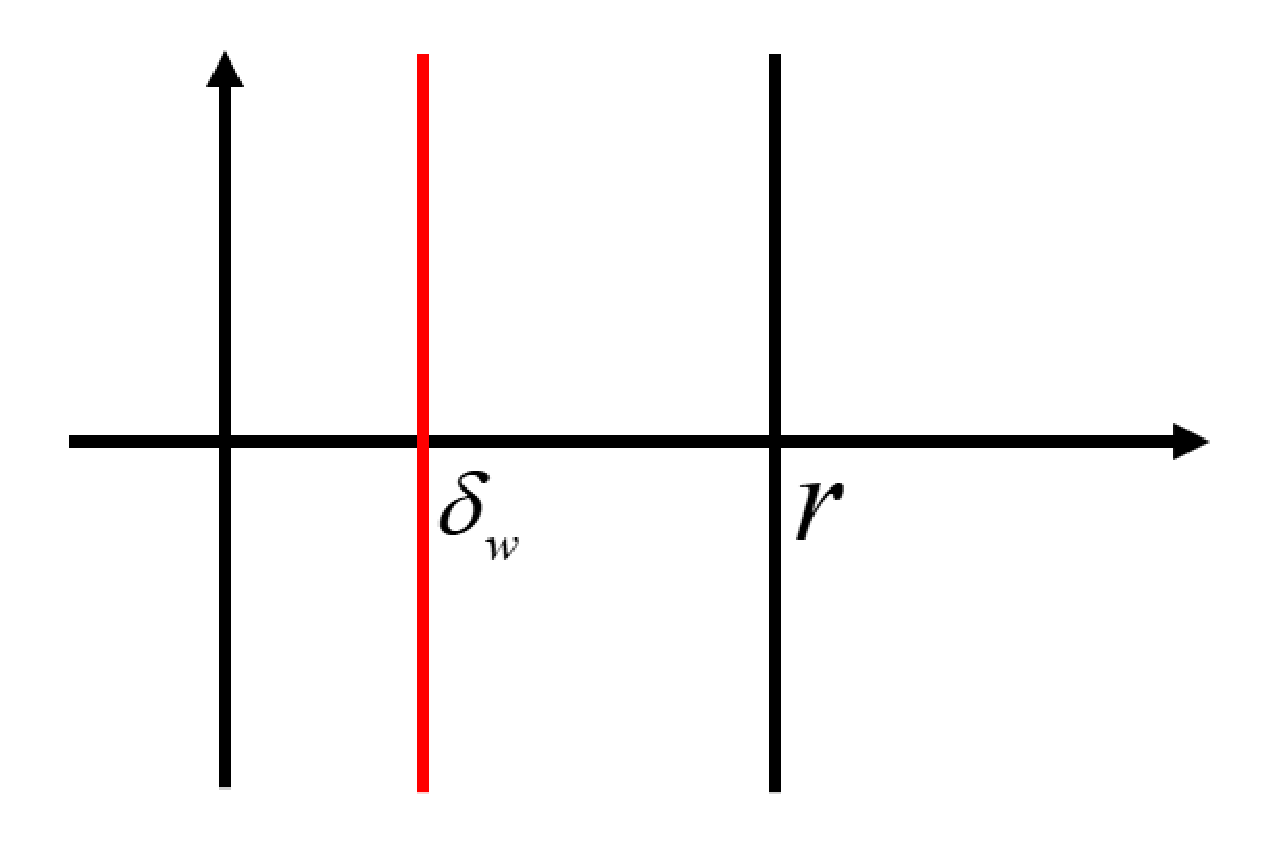
\includegraphics[width=8cm]{14.eps}
        \caption*{}
    \end{figure}
    解得:$\displaystyle\psi(x, y)=\frac{r}{\beta}\left[1-\frac{2}{\sqrt{3}} e^{-\frac{1}{2} k x} \cos \left(\frac{\sqrt{3}}{2} k x-\frac{\pi}{6}\right)\right] \frac{\partial \tau_{x \zeta}}{\partial y} $\\
    \paragraph{东边界区}~{}
    $$\psi(x, y)=\frac{r}{\beta}\left[1-\frac{x}{r}+\frac{1}{k r}\left(e^{-k(r-x)}-1\right)\right] \frac{\partial \tau_{x \zeta}}{\partial y} $$\\
    综合内区、西边界区和东边界区的解可得统一的解的形式:
    \[
        \color{red}
        \boxed{
            \psi=\frac{r}{\beta} f(x) \frac{\partial x_{x \zeta}}{\partial y}
        }
    \]
    \paragraph{讨论}~{}
    \paragraph{环流空间分布特征}~{\centering 图片来自$Introduction \;to \; Physical \;Oceanography$(Robert H. Stewart,2008 pp191)}
    \begin{figure}[H]
        \centering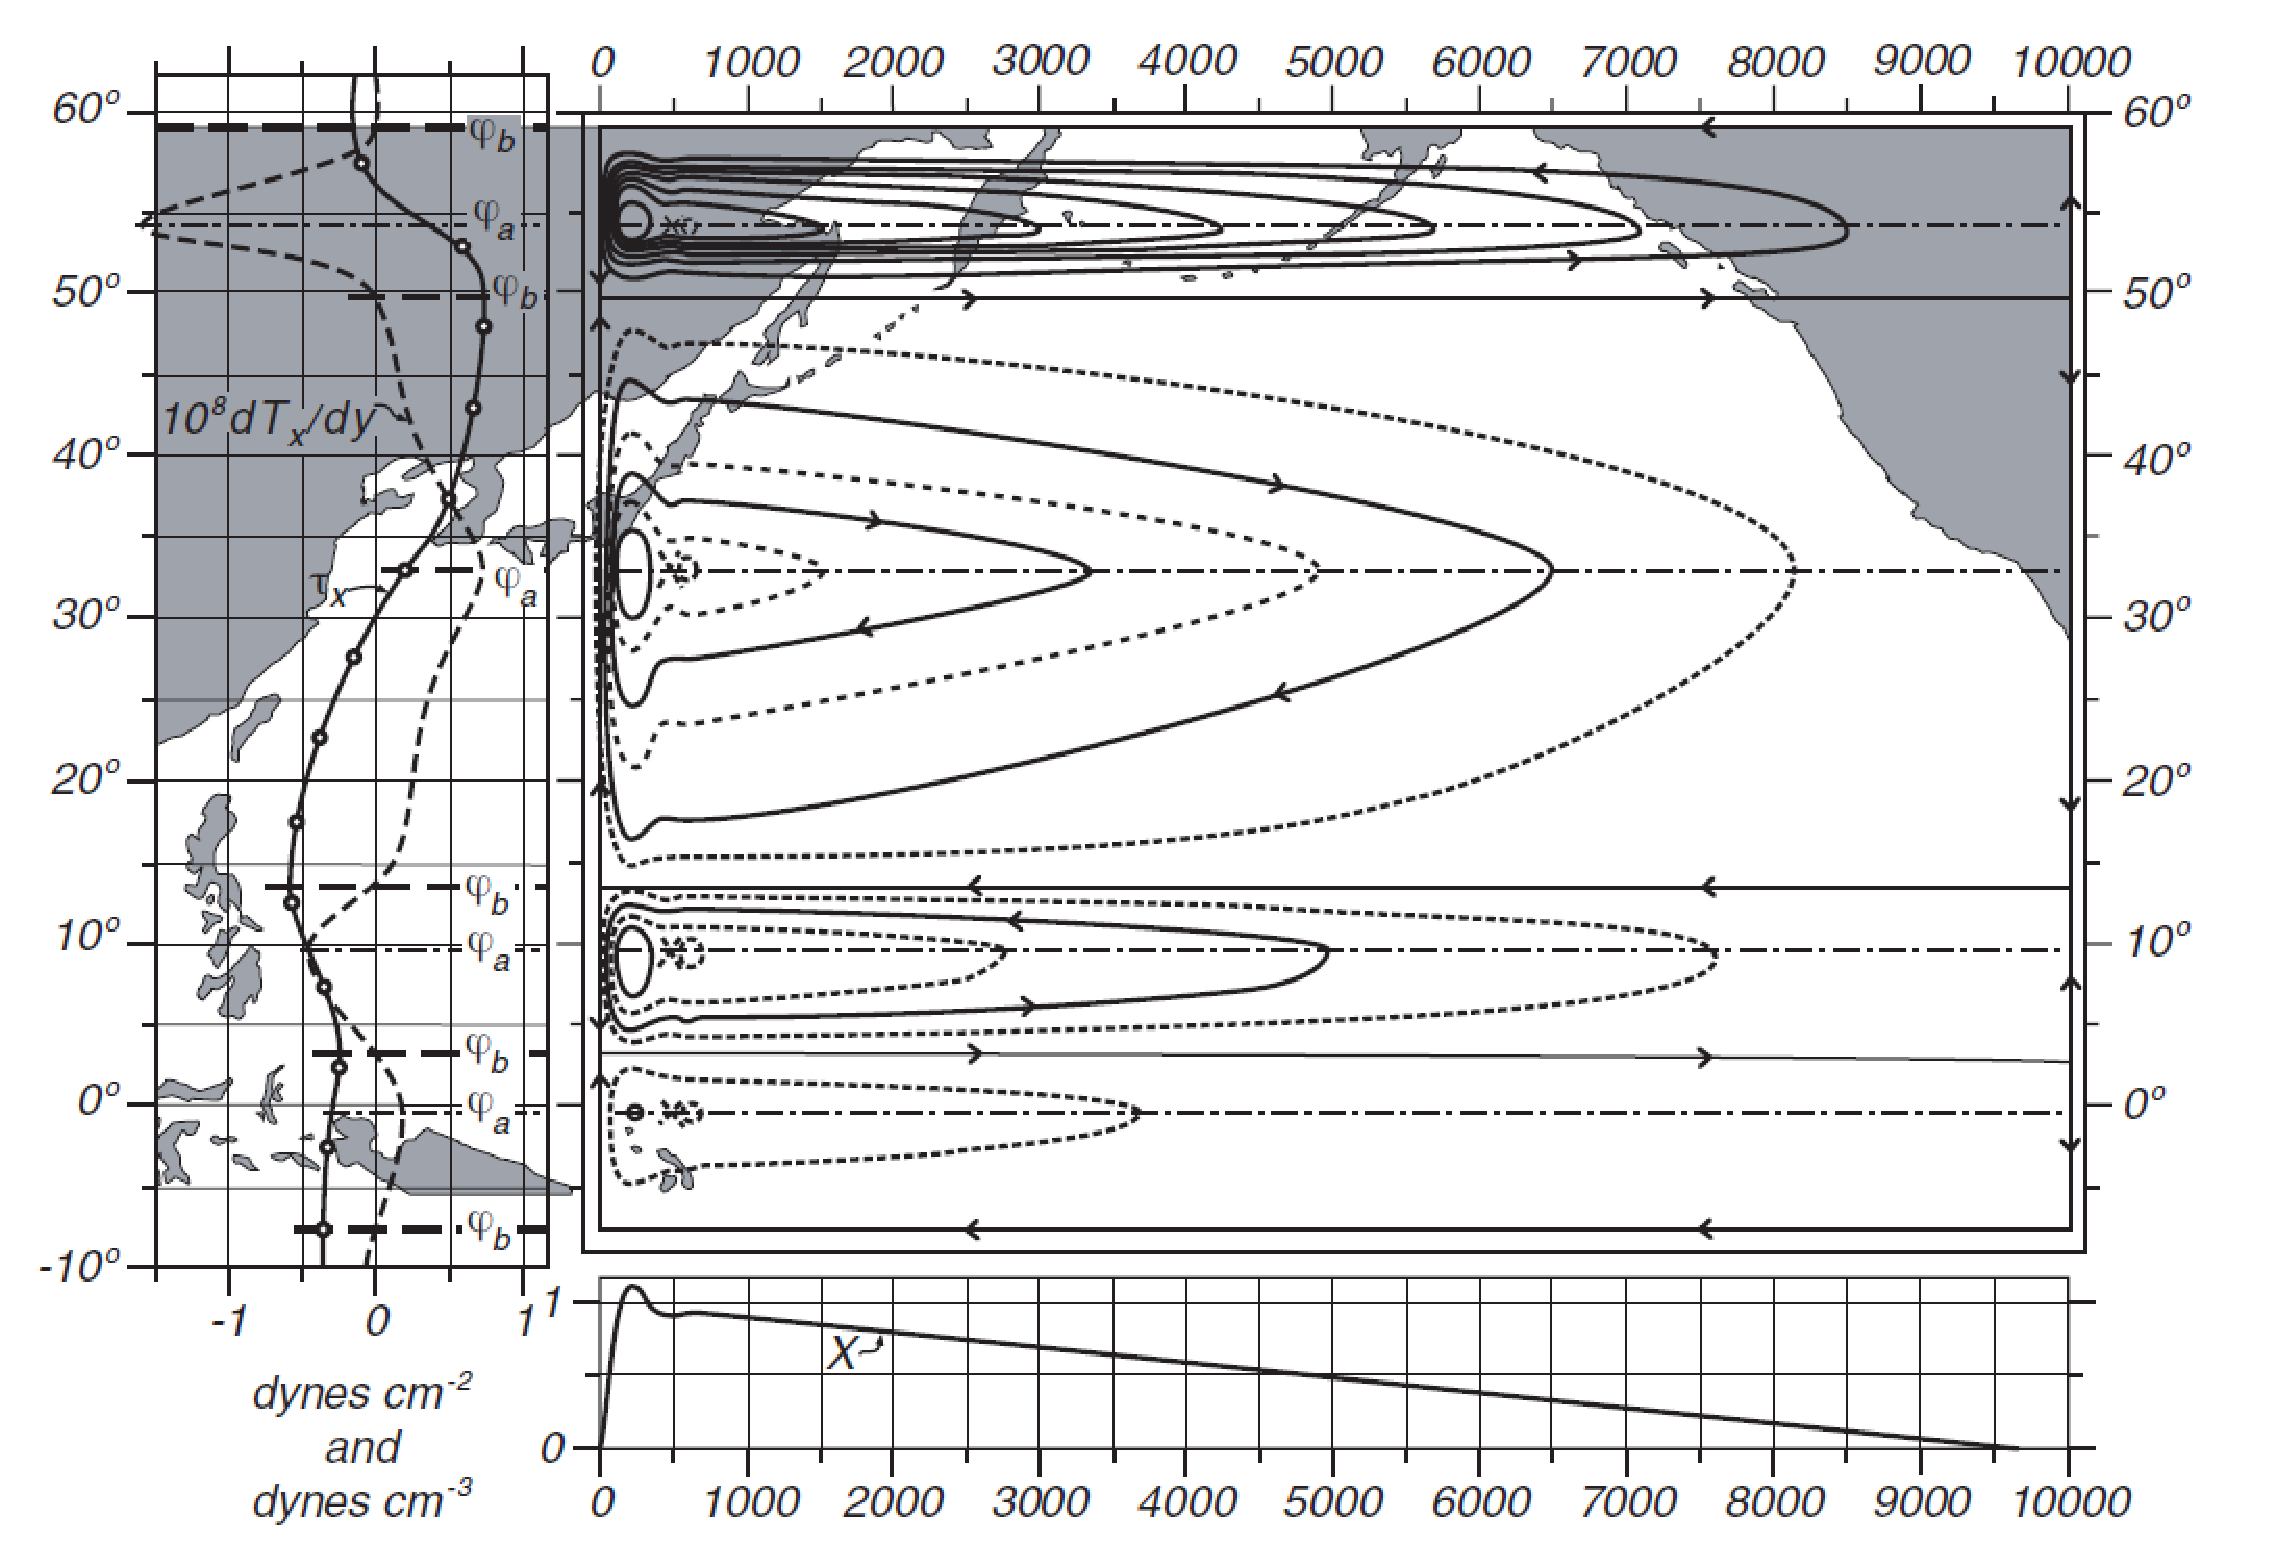
\includegraphics[width=13cm]{15.eps}
        \caption*{}
    \end{figure}
    (1) Gyres之间的分界处位于:$\displaystyle M_y=\frac{\partial \psi}{\partial x}=0$,只有东西向的流动:$\displaystyle f^{\prime}(x)=0/\frac{\partial \tau_{x\zeta}}{\partial y}=0$;\\
    (2) Gyres主轴位于:$\displaystyle M_x=\frac{\partial \psi}{\partial x}=0$只有南北向的流动:$\displaystyle f(x)=0/\frac{\partial^2 \tau_{x\zeta}}{\partial y^2}=0$;\\
    (3) 流动西强东弱.
    \paragraph{大洋西边界区的物质输运特点}~{}
    \[
        \psi_{W}=\frac{r}{\beta} f_{m}(x) \frac{\partial \tau_{x \zeta}}{\partial y}
    \]
    质量输运:
    \[
        \left\{
            \begin{aligned}
                &M_{xW}=-\frac{\partial \psi}{\partial y}=-\frac{r}{\beta} f_{W}(x) \frac{\partial^{2} \tau_{x \zeta}}{\partial y^{2}}\\
                &M_{yW}=\frac{\partial \psi}{\partial x}=\frac{r}{\beta} f_{W}^{\prime}(x) \frac{\partial \tau_{x \zeta}}{\partial y}
            \end{aligned}
        \right.
    \]
    其中,$\displaystyle\left\{\begin{aligned}&f_{W}(x)=1-\frac{2}{\sqrt{3}} e^{-\frac{1}{2} k x} \cos \left(\frac{\sqrt{3}}{2} k x-\frac{\pi}{6}\right)\\&f_{W}^{\prime}(x)=\frac{2}{\sqrt{3}} k e^{-\frac{1}{2} k x} \sin \frac{\sqrt{3}}{2} k x\end{aligned}\right.$
    \begin{figure}[H]
        \centering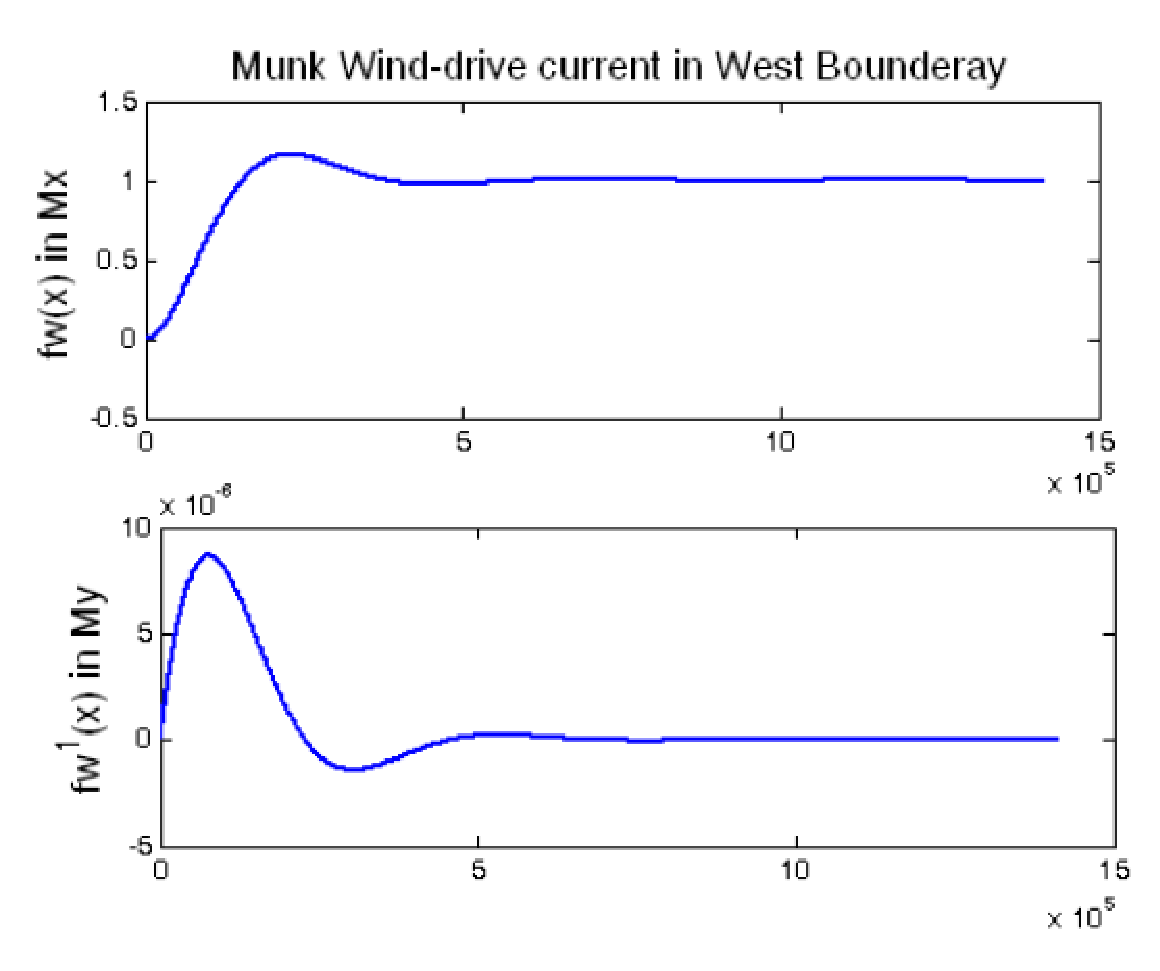
\includegraphics[width=13cm]{16.eps}
        \caption*{\large 随$x$增大而衰减的阻尼振动}
    \end{figure}
    对于任意纬度:
    \[
        M_{y W}=\frac{\partial \psi}{\partial x}=\frac{r}{\beta} f_{w}^{\prime}(x) \frac{\partial \tau_{x \zeta}}{\partial y}
    \]
    因此,$\displaystyle f_W^{\prime}(x)$的极值决定了$\displaystyle M_{yW}$的极值:
    \[
        \begin{aligned}
            &f_W^{\prime\prime}(x)=0 \\
            (\mbox{令}\lambda_W=\frac{2\pi}{\mbox{波数}}=\frac{4\pi}{\sqrt{3}k})
            \Rightarrow &x_{a, b}=\frac{2 \pi}{3 \sqrt{3} k}\left(\frac{1}{6} \lambda_{W}\right), \quad \frac{8 \pi}{3 \sqrt{3} k}\left(\frac{4}{6} \lambda_{W}\right)\\
            \Rightarrow &
            \left\{\begin{aligned}
                &f_{W}^{\prime}\left(x_{a}\right)=k e^{-\pi / 3 \sqrt{3}}\\
                &f_{W}^{\prime}\left(x_{b}\right)=-k e^{-4\pi / 3 \sqrt{3}}
            \end{aligned}\right.
        \end{aligned}
    \]
    \[
        \frac{f_{W}^{\prime}\left(x_{b}\right)} { f_{W}^{\prime}\left(x_{a}\right)}=-e^{-\pi / 3}=-0.17
    \]
    在西边界内,以$x=x_a$(1/6)波长为主轴处有一主流为北向的流动;以$x=x_b$(4/6)波长为主轴处存在一逆流,逆流的量值为主流的0.17倍.\\
    对于任意给定纬度,$\displaystyle f_W(x)$的极值决定$\displaystyle M_{xW}$的极值:
    \[
        f_W^{\prime}(x)=0\Rightarrow x_{1,2}=\frac{2\pi}{\sqrt{3}k},\frac{4\pi}{\sqrt{3}k}\Rightarrow \left\{\begin{aligned}
            &f_{W}\left(x_{1}\right)=1-e^{-\pi/\sqrt{3}}\\
            &f_{W}\left(x_{2}\right)=1+e^{-2\pi/\sqrt{3}}
        \end{aligned}\right.
    \]
    极值在1附近变动.
    \paragraph{缺陷}~{}\\
    (1) 若取$\displaystyle A_l=5\times 10^3 m^2s^{-1}$,西部阻尼振荡的波长比实际大约3倍:$\displaystyle \lambda=\frac{4\pi}{\sqrt{3}k}=\frac{4\pi}{\sqrt{3}}\frac{1}{\sqrt[3]{\beta/A_l}}\approx 200km$;符合实际主流和逆流宽度时,$A_l=10^2m^2s^{-1}$\\
    (2) 西部总流量比实测值小一半.
    \section{海浪}
    \subsection{线性波动理论}
    理论框架:
    \begin{figure}[H]
        \centering 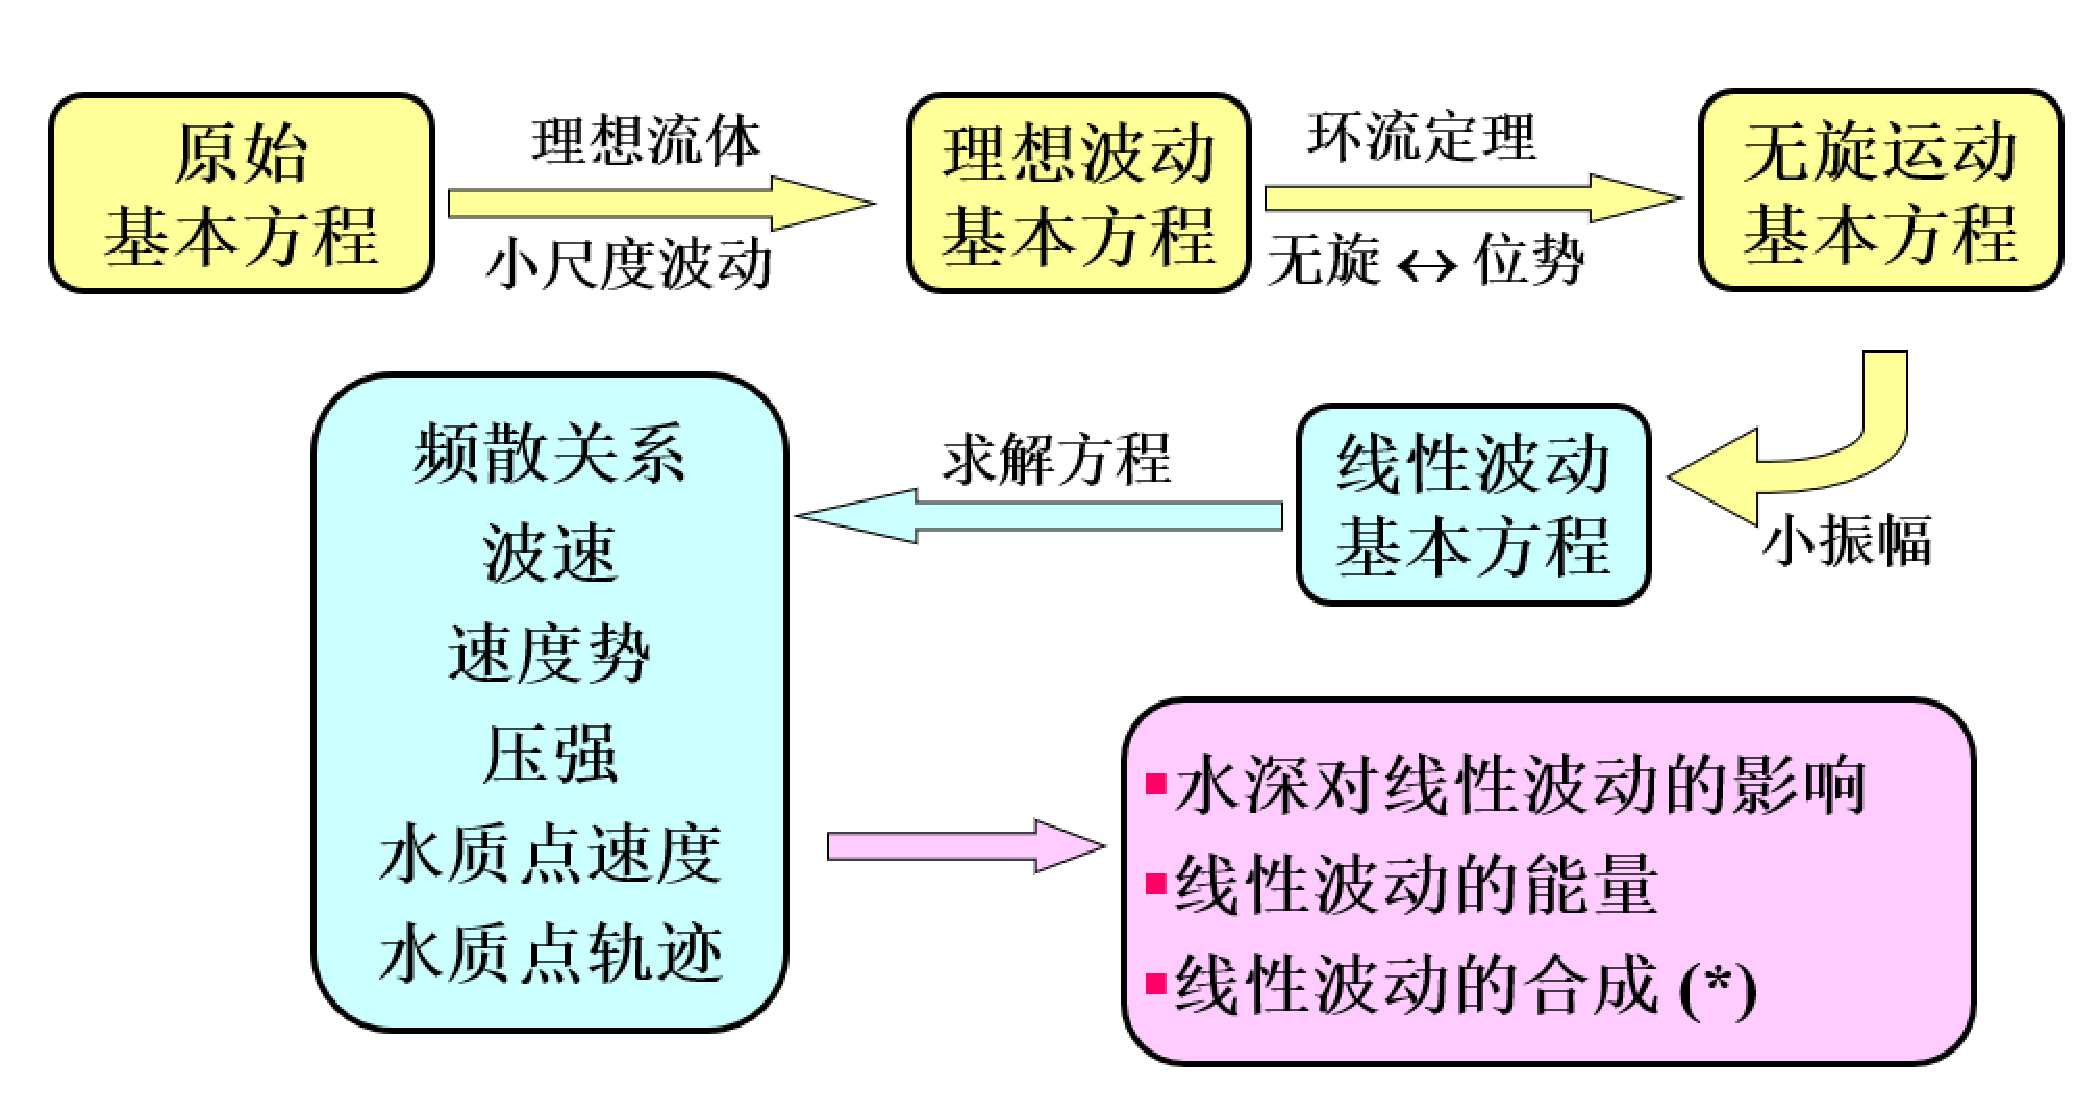
\includegraphics[width=11cm]{17.eps}
        \caption*{}
    \end{figure}
    \subsubsection{无旋运动的基本方程}
    \paragraph{假定及方程}~{}\\
    (1) 海水均匀不可压缩;\\
    (2) 理想流体;\\
    (3) 短周期小尺度波动;\\
    (4) 重力为唯一的外力;\\
    (5) 忽略分子粘性项、科氏力、引潮力和湍摩擦力.\\
    控制方程:
    \[
        \left\{
            \begin{aligned}
                &\frac{d\vec{V}}{dt}=\frac{\partial \vec{V}}{\partial t}+(\vec{V}\cdot\nabla)\vec{V}=-\frac{1}{\rho}\nabla p-\vec{g}\\
                &\frac{\partial u}{\partial x}+\frac{\partial v}{\partial y}+\frac{\partial w}{\partial z}
            \end{aligned}
        \right.
    \]
    边界条件:
    \[
        \left\{
            \begin{aligned}
                &z=\zeta(\mbox{海面}):{{\partial \zeta } \over {\partial t}} + u{{\partial \zeta } \over {\partial x}} + v{{\partial \zeta } \over {\partial y}} = w,p_I=p_a(x,y,t)\\
                &\mbox{固体边界处}:V_n=0
            \end{aligned}
        \right.
    \]
    \paragraph{环流定理}~{}
    \begin{figure}[H]
        \centering 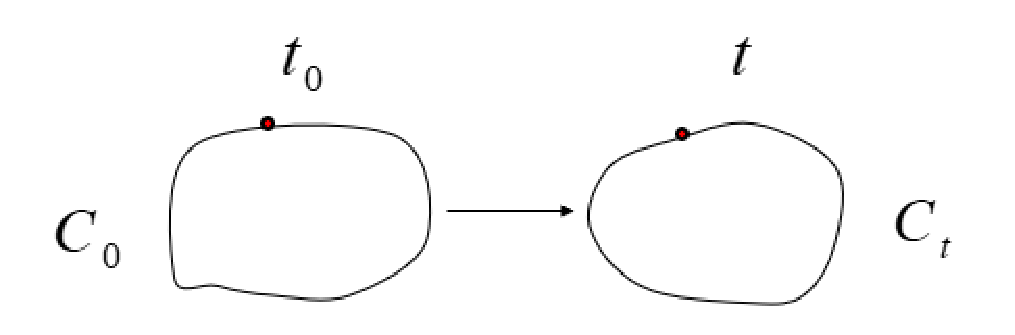
\includegraphics[width=7cm]{18.eps}
        \caption*{}
    \end{figure}
    $C_t$上的环流:$\displaystyle \Gamma(t)=\oint\limits_{ct}udx+vdy+wdz$
    \[
    \begin{aligned}
        &\Rightarrow \frac{d \Gamma(t)}{d t}=\oint\limits_{c t} \left(\frac{d u}{d t} d x+\frac{d v}{d t} d y+\frac{d w}{d t} d z\right)+\underbrace{\oint\limits_{c t} \left(u d u+v d v+w d w\right)}_{=\frac{1}{2} \oint\limits_{c t} d u^{2}+d v^{2}+d w^{2}=0}\\
        &\Rightarrow \frac{d \Gamma(t)}{d t}=\oint\limits_{c t} \frac{d \vec{V}}{d t} \cdot d \vec{l}
    \end{aligned}
    \]
    环流的实质微商等于加速度的环流.
    \[
        \frac{d \Gamma(t)}{d t}=\oint\limits_{c t}\left(-\frac{1}{\rho} \frac{\partial p}{\partial x}\right) d x+\left(-\frac{1}{\rho} \frac{\partial p}{\partial y}\right) d y+\left(-\frac{1}{\rho} \frac{\partial p}{\partial z}-g\right)d z=\oint\limits_{c t} d\underbrace{\left(-\frac{p}{\rho}-g z\right)}_{\mbox{单值函数}}=0 
    \]
    $\color{red}\mbox{环流定理}$:对不可压缩的理想流体,由相同质点构成的封闭曲线上的环流不随时间而变。
    \paragraph{无旋运动的基本方程和边界条件}~{}\\
    若在重力场中,理想流体于起始时刻为静止或匀速运动,则任何时刻,对任何封闭曲线有:$\Gamma(t)=0$,根据Stokes定理:
    \[
        \Gamma(t)=\oint\limits_{c t} \vec{V} \cdot d \vec{l}=\iint\limits_{s} \nabla \times \vec{V} d \sigma=0\Rightarrow\nabla\times\vec{V}=\Rightarrow\vec{V}=\nabla \varphi
    \]
    运动方程:
    \[
            \frac{d\vec{V}}{dt}=\frac{\partial \vec{V}}{\partial t}+(\vec{V}\cdot\nabla)\vec{V}=-\frac{1}{\rho}\nabla p-\vec{g}
    \]
    \[
        \begin{aligned}
            &\Rightarrow \frac{d\vec{V}}{dt}=\frac{\partial \vec{V}}{\partial t}+\frac{1}{2}\nabla(\vec{V}\cdot\vec{V})=-\nabla\frac{p-p_0}{\rho}-\nabla(gz)\\
            &\Rightarrow \nabla\frac{\partial \varphi}{\partial t}+\frac{1}{2}\nabla(\nabla\varphi\cdot\nabla\varphi)=-\nabla\frac{p-p_0}{\rho}-\nabla(gz)\\
            &\Rightarrow \frac{\partial \varphi}{\partial t}+\frac{1}{2}(\nabla \varphi)(\nabla \varphi)+\frac{p-p_{0}}{\rho}+g z=0
        \end{aligned}
    \]
    连续方程:
    \[
        \Delta \varphi=\frac{\partial^{2} \varphi}{\partial x^{2}}+\frac{\partial^{2} \varphi}{\partial y^{2}}+\frac{\partial^{2} \varphi}{\partial z^{2}}=0
    \]
    运动学边界条件: 
    \[
        \begin{aligned}
            \mbox{海面}:&\left.\left(\frac{\partial \zeta}{\partial t}+\frac{\partial \varphi}{\partial x} \frac{\partial \zeta}{\partial x}+\frac{\partial \varphi}{\partial y} \frac{\partial \zeta}{\partial y}\right)\right|_{z=\zeta}=\left.\frac{\partial \varphi}{\partial z}\right|_{z=\zeta} \\
            \mbox{固定边界}:&\frac{\partial \varphi}{\partial n}=0
        \end{aligned}
    \]
    动力学边界条件: 
    \[
        \begin{aligned}
            &p_{I}=p_{a}(x, y, t) \\
            &{\left.\left[\frac{\partial \varphi}{\partial t}+\frac{1}{2}(\nabla \varphi)(\nabla \varphi)\right]\right|_{z=\zeta}+g \zeta=0}
        \end{aligned}
    \]
    \subsubsection{线性波动}
    \paragraph{假定}~{}\\
    (1) 均质不可压理想流体;\\
    (2) 波动的振幅相对波长很小;\\
    (3) 设水域广阔等深;\\
    (4) 波动只沿x方向传播.\\
    小振幅假定$\displaystyle:\Rightarrow\left\{\begin{aligned}&\varphi\mbox{的微商乘积项可忽略}\\&\left.\left.\frac{\partial \varphi}{\partial z}\right|_{z=\zeta} \approx \frac{\partial \varphi}{\partial z}\right|_{z=0},\left.\left.\frac{\partial \varphi}{\partial t}\right|_{z=\zeta} \approx \frac{\partial \varphi}{\partial t}\right|_{z=0}\end{aligned}\right.$
    \paragraph{方程简化}~{}\\
    \begin{spacing}{2}
        运动方程:$\displaystyle \frac{\partial \varphi}{\partial t}+\cancel{\frac{1}{2}(\nabla \varphi)(\nabla \varphi)}+\frac{p-p_{0}}{\rho}+g z=0$\\
    连续方程:$\displaystyle\Delta \varphi=\frac{\partial^{2} \varphi}{\partial x^{2}}+\cancel{\frac{\partial^{2} \varphi}{\partial y^{2}}}+\frac{\partial^{2} \varphi}{\partial z^{2}}=0$\\
    边界条件:$\displaystyle \left\{\begin{aligned}
        &\left.\left(\frac{\partial \zeta}{\partial t}+\cancel{\frac{\partial \varphi}{\partial x} \frac{\partial \zeta}{\partial x}+\frac{\partial \varphi}{\partial y} \frac{\partial \zeta}{\partial y}}\right)\right|_{z=\zeta}=\left.\frac{\partial \varphi}{\partial z}\right|_{z=\zeta} \\
        &\frac{\partial \varphi}{\partial n}=\left.0 \Rightarrow \frac{\partial \varphi}{\partial z}\right|_{z=-d}=0 \\
        &{\left.\left[\frac{\partial \varphi}{\partial t}+\cancel{\frac{1}{2}(\nabla \varphi)(\nabla{\varphi})}\right]\right|_{z=\zeta}+g \zeta=0}
        \end{aligned}\right.$
    \end{spacing}
    因此,$\color{red}\mbox{线性波动的基本方程}$:
    \begin{numcases}{}
        \frac{\partial \varphi}{\partial t}+\frac{p-p_{0}}{\rho}+g z=0 \label{lw1}\\
        \frac{\partial^{2} \varphi}{\partial x^{2}}+\frac{\partial^{2} \varphi}{\partial z^{2}}=0 \label{lw2}\\
        \left.\frac{\partial \varphi}{\partial z}\right|_{==0}=\frac{\partial \zeta}{\partial t}\label{lw4} \\
        \left.\frac{\partial \varphi}{\partial z}\right|_{z=-d}=0 \label{lw4}\\
        \left.\frac{\partial \varphi}{\partial t}\right|_{z=0}+g \zeta=0\label{lw5}
    \end{numcases}
    $(\ref{lw5})$代入$(\ref{lw3})$中:
    \[
        \left.\left(\frac{\partial \varphi}{\partial z}+\frac{1}{g} \frac{\partial^{2} \varphi}{\partial t^{2}}\right)\right|_{z=0}=0\label{lw6}
    \]
    \paragraph{求解}~{}\\
    对前进波:
    \begin{equation}
        \varphi=\varphi_0(z)\cos(kx-\omega t) \label{*}
    \end{equation}
    $(\ref{*})$代入$(\ref{lw2})$中:
    \begin{equation}
        \varphi_0(z)=Ae^{kz}+Be^{-kz} \label{lw7}
    \end{equation}
    $(\ref{*})$代入$(\ref{lw6})$中(海面):
    \begin{equation}
        \left.\left[\frac{\partial \varphi_{0}(z)}{\partial z}-\frac{\omega^{2}}{g} \varphi_{0}(z)\right]\right|_{z=0}=0 \label{lw8}
    \end{equation}
    $(\ref{*})$代入$(\ref{lw4})$中(海底):
    \begin{equation}
        \left.\frac{d \varphi_{0}(z)}{d z}\right|_{z=-d}=0\label{lw9}
    \end{equation}
    $(\ref{lw7})$代入$(\ref{lw8})$中:
    \begin{equation}
            \left(\omega^{2}-g k\right) A+\left(\omega^{2}+g k\right) B =0 \label{lw10}
    \end{equation}
    $(\ref{lw7})$代入$(\ref{lw9})$中:
    \begin{equation}
        e^{-k d} A-e^{k d} B =0 \label{lw11}
    \end{equation}
    联立$(\ref{lw10}),(\ref{lw11})$,有非零解的条件为:
    \[
        \left|\begin{array}{cc}
            e^{-k d} & -e^{k d} \\
            \left(\omega^{2}-g k\right) & \left(\omega^{2}+g k\right)
            \end{array}\right|=0\Rightarrow \color{red}\mathop{\omega^2=gk\operatorname{th} kd}\limits_{\color{red}\mbox{频散关系}}
    \]
    频散关系表示波动频率和波数之间的关系,代表某种波动的性质.\\
    波速:$\displaystyle c=\frac{\lambda}{T}=\frac{2 \pi / k}{2 \pi / \omega}=\frac{\omega}{k} \Rightarrow c^{2}=\frac{\omega^{2}}{k^{2}}=\frac{g}{k} \text { th } k d $\\
    波速与水深和波动性质有关系.\\
    由$(\ref{lw11}):A e^{-k d}=B e^{k d}=\frac{1}{2} D\Rightarrow A=\frac{D}{2} / e^{-k d} ; \quad B=\frac{D}{2} / e^{k d}$\\
    代入$(\ref{*})$:
    \begin{equation}
        \varphi=D\operatorname{ch}[k(z+d)]\cos (kx-\omega t) \label{lw12}
    \end{equation}
    $(\ref{lw12})$代入$(\ref{lw5})$中:
    \[
        \zeta=-\frac{\omega}{g} D \operatorname{ch} k d  \sin (k x-\omega t)=a\sin (kx-\omega t)
    \]
    速度势的解:
    \begin{equation}
        \varphi=-\frac{a g}{\omega} \frac{\operatorname{ch}[k(z+d)]}{\operatorname{ch} k d} \cos (k x-\omega t) \label{lw13}
    \end{equation}
    $(\ref{lw13})$代入$(\ref{lw1})$中,可得压强分布:
    \[
        p=p_{0}+\rho g a \frac{\operatorname{ch}[k(z+d)]}{\operatorname{ch} k d} \sin (k x-\omega t)-\rho g z
    \]
    水质点速度:
    \[
        \begin{aligned}
            &u=\frac{\partial \varphi}{\partial x}=\frac{a g k}{\omega} \frac{\operatorname{ch}[k(z+d)]}{\operatorname{ch} k d} \sin (k x-\omega t) \\
            &w=\frac{\partial \varphi}{\partial z}=-\frac{{agk}}{\omega} \frac{\operatorname{sh}[k(z+d)]}{\operatorname{ch} k d} \cos (k x-\omega t)
            \end{aligned}
    \]
    水质点运动轨迹($x_0,z_0$)为平衡位置:
    \[
        \frac{\left(x-x_{0}\right)^{2}}{\left[a \frac{\operatorname{ch}\left[k\left(d+z_{0}\right)\right]}{\operatorname{sh} k d}\right]^{2}}+\frac{\left(z-z_{0}\right)^{2}}{\left[a \frac{\operatorname{sh}\left[k\left(d+z_{0}\right)\right]}{\operatorname{sh} k d}\right]^{2}}=1
    \]
    \paragraph{解的讨论}~{}
    \begin{figure}[H]
        \centering 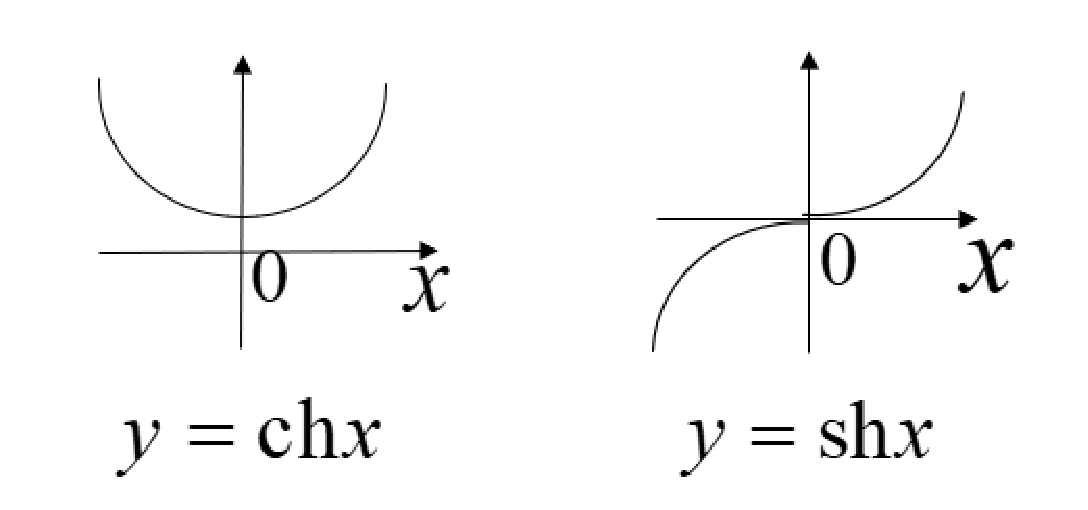
\includegraphics[width=8cm]{19.eps}
        \caption*{}
    \end{figure}
    (1) 线性波动水质点轨迹为椭圆,长轴为x方向;\\
    (2) 椭圆长轴和短轴均与z0 有关,与 x0 无关;\\  
    (3) 长轴和短轴均随平衡位置的加深而减小;\\
    (4) 在海底水质点做水平运动.

    \bibliographystyle{apalike}
	\bibliography{ref}
\end{document}